%% LaTeX Beamer presentation template (requires beamer package)
%% see http://bitbucket.org/rivanvx/beamer/wiki/Home
%% idea contributed by H. Turgut Uyar
%% template based on a template by Till Tantau
%% this template is still evolving - it might differ in future releases!

\documentclass{beamer}

\mode<presentation>

\usetheme{Malmoe}
\useoutertheme{infolines}
\useinnertheme{default}
\setbeamercovered{transparent}
\setbeamertemplate{footline}[frame number] % frame number in footline
\setbeamertemplate{itemize items}[circle]  % itemize circles
\renewcommand\textbullet{\ensuremath{\bullet}}  % no error for bullets
\setbeamertemplate{caption}[numbered]      % numbered captions
\beamertemplatenavigationsymbolsempty

% PACKAGES + MODIFICATIONS

\usepackage[ngerman]{babel} %language and fonts
\usepackage[utf8]{inputenc}
\usepackage{lmodern}
\usepackage{textgreek}

\usepackage{amsmath}  % math
\usepackage{amssymb}
\usepackage{mathptmx}

\usepackage{graphicx} %graphics
\usepackage{float} 
\graphicspath{{../img/}}

\usepackage{enumerate} % better way to config enumerates

\usepackage{multirow}  % multi rows in tables

\usepackage{hhline}  % for doule lines in table without interrupting vertical lines

\setbeamerfont{standard}{size=\normalsize}


% NEW COMMANDS
\newcommand{\abs}[1]{\left|#1\right|}
\newcommand{\rb}[1]{$^{#1}$\!Rb}
\newcommand{\difd}{\mathrm{d}}

% DOCUMENT SETTINGS


\title{Optisches Pumpen}
\subtitle{Fortgeschrittenen-Praktikum II}
\author{Moritz Bitterling \and Benjamin Rottler}
\institute[Universities of]{Universität Freiburg}
\date{18.05.2015}


% This is only inserted into the PDF information catalog. Can be left
% out.
\subject{Optisches Pumpen}

\AtBeginSection[]
{
\begin{frame}<beamer>
\frametitle{}
\tableofcontents[currentsection,hideothersubsections]
\end{frame}
}

\begin{document}

\begin{frame}
\titlepage
\end{frame}

\begin{frame}
\frametitle{Inhalt}
\tableofcontents[hideallsubsections]
\end{frame}

%%% BEN 5' %%%

\section{Allgemeine Grundlagen}

\subsection{Die Hyperfeinstruktur}

\begin{frame}
\frametitle{Hyperfeinstruktur-Aufspaltung}
\begin{itemize}
    \item<1-> Kopplung von Kernspin $\vec{I}$ und elektronischem Gesamtdrehimpuls $\vec{J}$
    \begin{equation*}
        \vec{F} = \vec{I} + \vec{J} \qquad \qquad \abs{I - J} \leq F \leq \abs{I + J}
    \end{equation*}
    \item<2-> Energieaufspaltung
    \begin{equation*}
        \Delta E_\text{HFS} = - \vec{\mu}_I \cdot \vec{B}_J
    \end{equation*}
    \item<3-> Für benachbarte Energieniveaus
    \begin{equation*}
        \Delta E_{\Delta F = 1} (F) = A(F+1)
    \end{equation*}
    Intervallkonstante $A$
\end{itemize}
\end{frame}


\begin{frame}
\frametitle{Hyperfeinstruktur-Aufspaltung von Rubidium}
\setbeamerfont{myfont}{size*=80}
\usebeamerfont{myfont}

\begin{figure}
    \centering
    \def\svgwidth{\textwidth}
    \input{../img/termschemahyperfein.pdf_tex}
    \caption{Hyperfeinstrukturaufspaltung der D$_1$-Linie von \rb{85} und \rb{87}.}
\end{figure}
\end{frame}


\begin{frame}
\frametitle{Hyperfeinstruktur-Aufspaltung - Übergänge}
\setbeamerfont{myfont}{size*=80}
\usebeamerfont{myfont}

\begin{figure}
    \centering
    \def\svgwidth{\textwidth}
    \input{../img/termschemahyperfein_linien.pdf_tex}
    \caption{Hyperfeinstrukturaufspaltung der D$_1$-Linie von 
    \rb{85} und \rb{87}.}
\end{figure}
\end{frame}

 


\begin{frame}
\frametitle{Hyperfeinstruktur-Aufspaltung - Spektrallinien}
\setbeamerfont{myfont}{size*=80}
\usebeamerfont{myfont}

\begin{figure}
    \centering
    \def\svgwidth{\textwidth}
    \input{../img/HFSspect_theo.pdf_tex}
    \caption{Spektrallinien der Hyperfeinstruktur des ${}^2\text{S}_{1/2}$\,-\,${}^2\text{P}_{1/2}$\,-\,Übergangs
    von \rb{85} und \rb{87}.}
\end{figure}

\end{frame}

\begin{frame}
\frametitle{Zeeman-Aufspaltung der Hyperfeinstruktur}
\begin{itemize}
    \item<1-> ohne Magnetfeld: Niveau ist $(2F+1)$-fach entartet
    \begin{equation*}
        F_z = m_F \hbar \qquad \qquad -F \leq m_F \leq F
    \end{equation*}
    \item<2-> mit äußerem Magnetfeld $\vec{B}_0$: Zeeman-Aufspaltung
    \item<3-> Für benachbarte Energieniveaus
    \begin{equation*}
        \Delta E_\text{HFS}^\text{Zeeman}(\Delta m_F = 1) = \frac{g_J \mu_B}{2 \left( I + \frac{1}{2} \right) } B_0
    \end{equation*}
    Bohrsches Magneton $\mu_B$, Landé-Faktor $g_J$
\end{itemize}
\end{frame}

\begin{frame}
\frametitle{Zeeman-Aufspaltung der Hyperfeinstruktur}

\setbeamerfont{myfont}{size*=80}
\usebeamerfont{myfont}

\begin{figure}
    \centering
    \def\svgwidth{\textwidth}
    \input{../img/termschema.pdf_tex}
    \caption{Zeeman-Aufspaltung der Hyperfeinstruktur von \rb{85} und \rb{87}.}
\end{figure}

\end{frame}




%%% MORITZ 2.5' %%%

\subsection{Die Laserdiode}

\begin{frame}
\frametitle{Laserdiode - Aufbau zur Charakterisierung}
\setbeamerfont{myfont}{size*=80}
\usebeamerfont{myfont}
\begin{figure}
    \centering
    \def\svgwidth{\textwidth}
    \input{../img/aufbauLaser.pdf_tex}
    \caption{Aufbau zur Messung der $P$-$I$-Kennlinie der Laserdiode.}
\end{figure}
\usebeamerfont{standard}
\begin{itemize}
  \item \textbf{Peltierelement:} Temperaturstabilisierung der Laserdiode
  \item \textbf{Laserdiode:} Erzeugung von linear polarisiertem kohärenten Licht mit $\lambda=500$\,nm
  \item \textbf{Neutraldichtefilter:} Abschwächung der Laserintensität
  \item \textbf{Photodiode:} Messung der Laserintensität
\end{itemize}
\end{frame}

\begin{frame}
\frametitle{Laserdiode - $P$-$I$-Kennlinie}

\begin{figure}[H]
    \begin{center}
        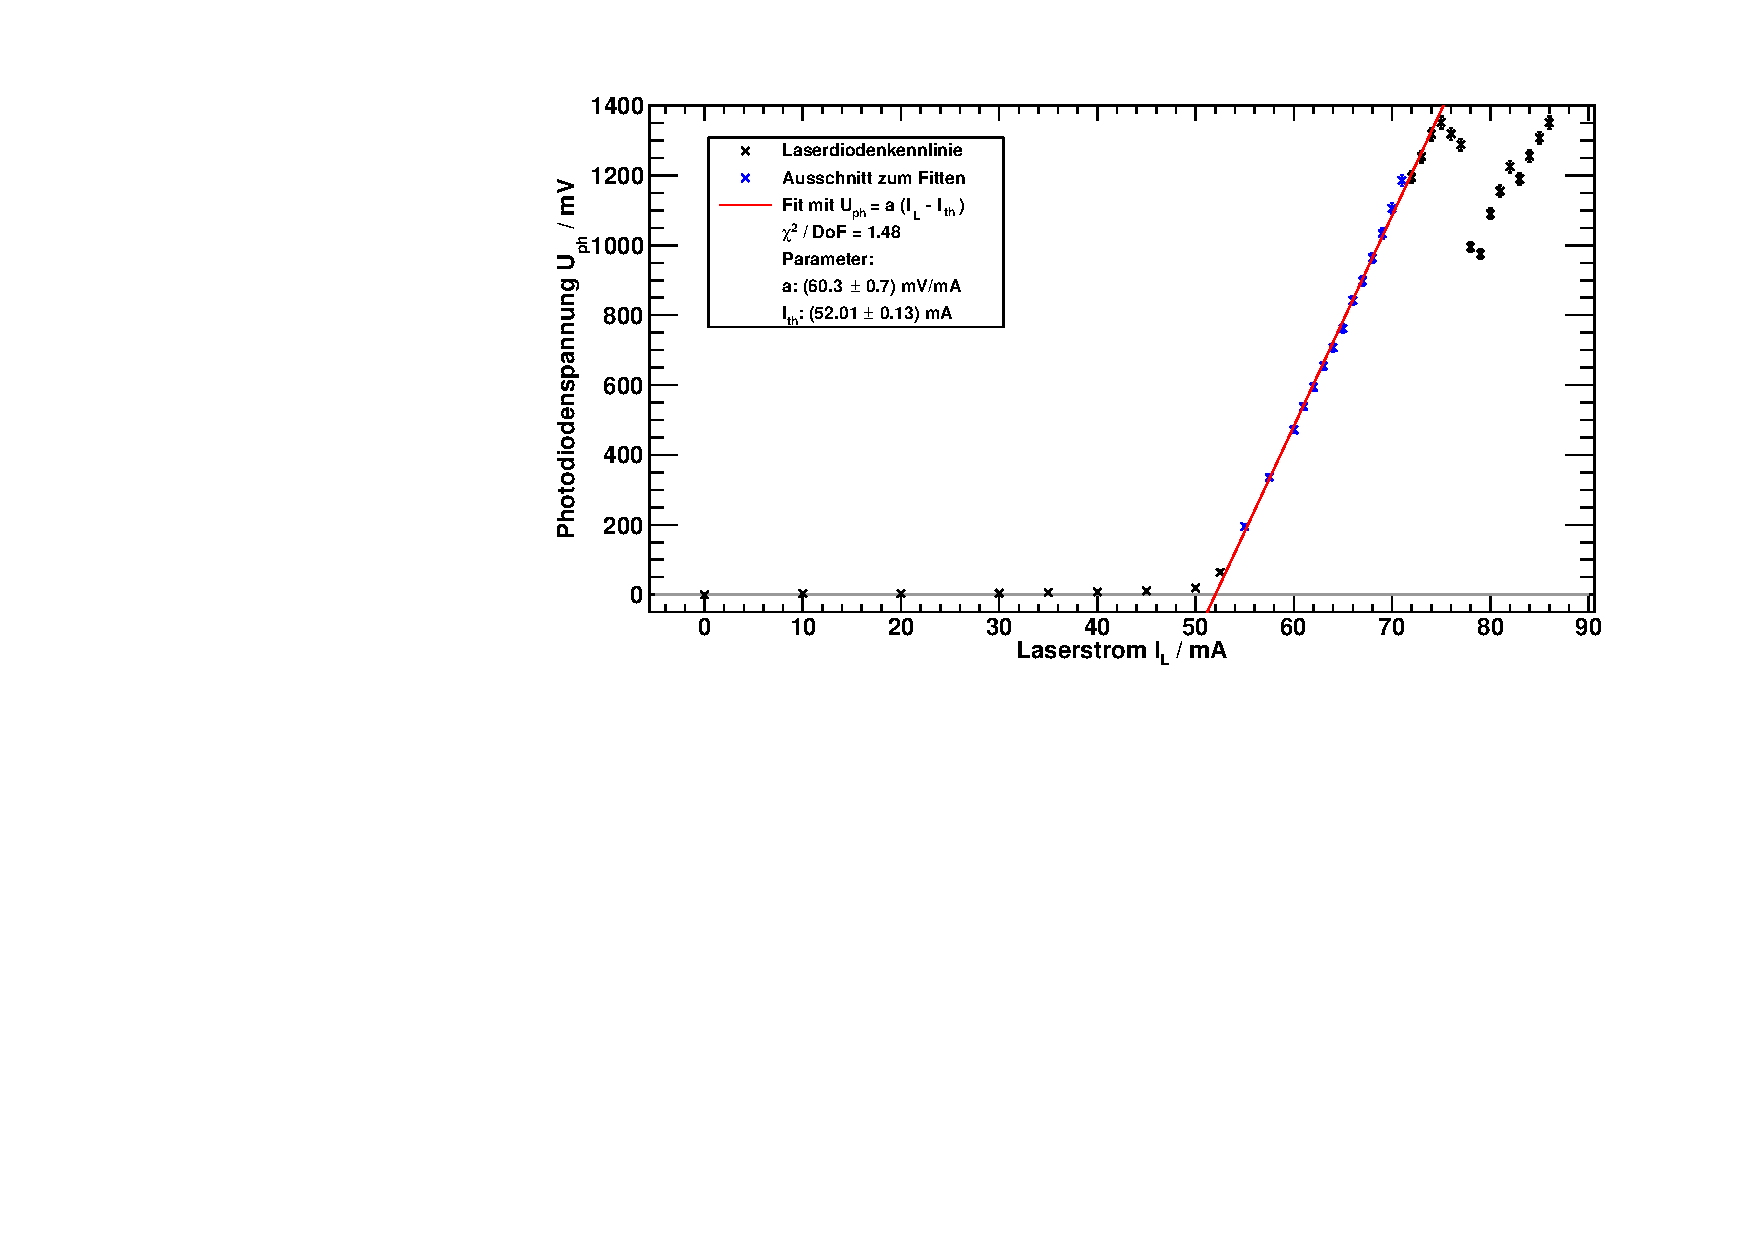
\includegraphics[width=\textwidth]{../img/diodenkennlinie.pdf}
        \caption{$P$-$I$-Kennlinie der im Versuch verwendeten Laserdiode.}
    \end{center}
\end{figure}
\end{frame}


\begin{frame}
\frametitle{Laserdiode - Aufbau zur Charakterisierung}
\setbeamerfont{myfont}{size*=80}
\usebeamerfont{myfont}
\begin{figure}
    \centering
    \def\svgwidth{\textwidth}
    \input{../img/aufbauEtalon.pdf_tex}
    \caption{Aufbau zur Identifikation von Modensprüngen der Laserdiode.}
\end{figure}
\usebeamerfont{standard}
\begin{itemize}
  \item \textbf{Etalon:} Transmissionsmaxima mit bekanntem Abstand
\end{itemize}
\end{frame}


\begin{frame}
\frametitle{Laserdiode - Frequenzmodulation}
\begin{figure}[H]
    \begin{center}
        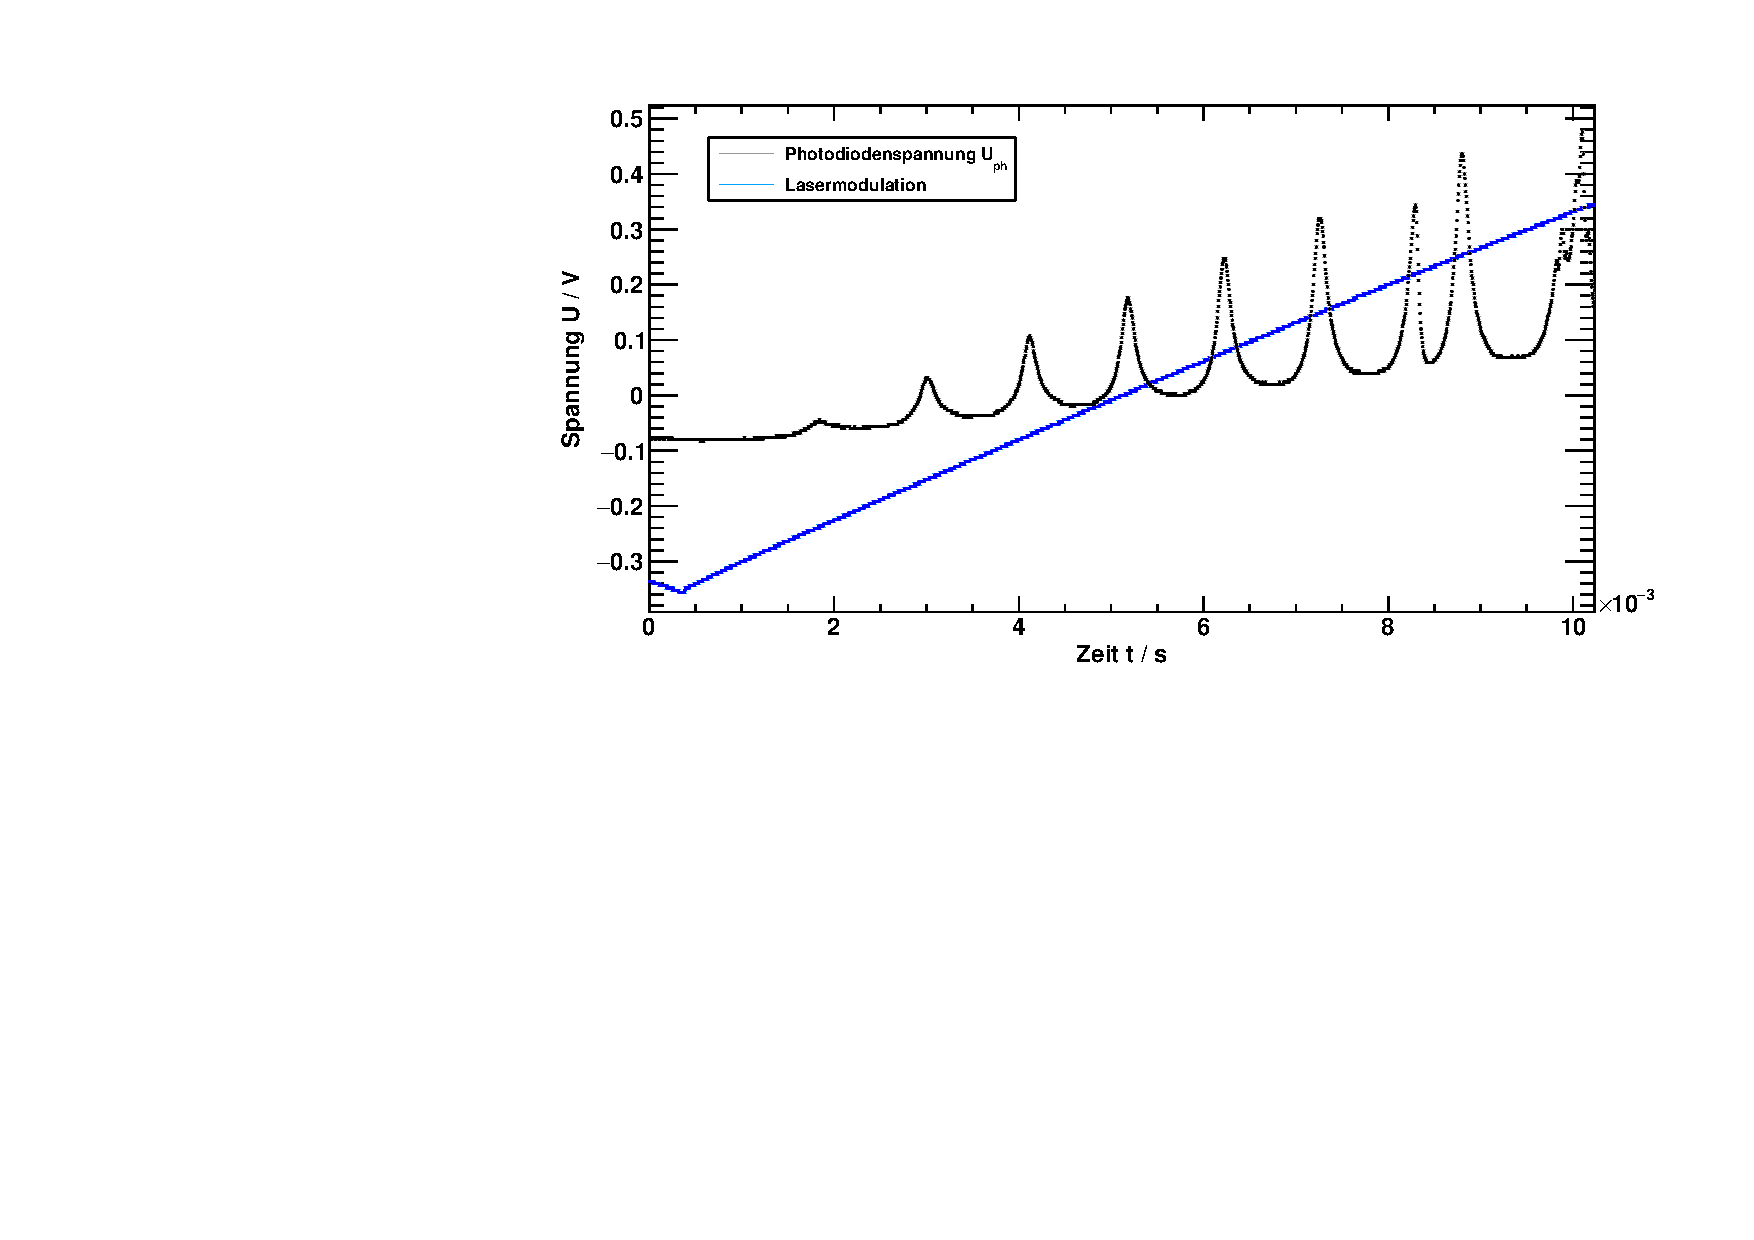
\includegraphics[width=\textwidth]{../img/up-etalon_zoom.pdf}
        \caption{Frequenzabhängige Transmission des Laserlichts durch das Etalon.}
    \end{center}
\end{figure}
\end{frame}


\begin{frame}
\frametitle{Laserdiode - Frequenzmodulation}

\begin{figure}[H]
    \begin{center}
        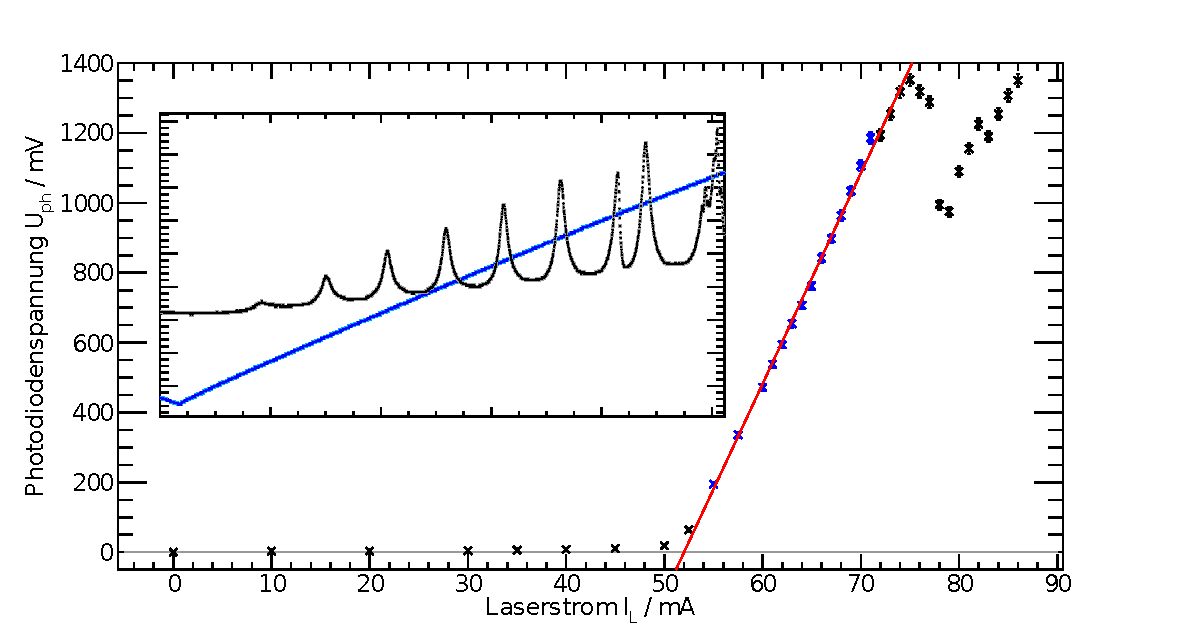
\includegraphics[width=\textwidth]{../img/diodenkennlinie+etalonspect.pdf}
        \caption{Vergleich von Frequenz und Leistung der Laserdiode.}
    \end{center}
\end{figure}
\end{frame}




%\section{Laser}
\subsection{Aufbau}
\begin{frame}
\frametitle{Laser}
  
\end{frame}

\subsection{Kennlinie}

\begin{frame}
\frametitle{Kennlinie}
  
\end{frame}
\section{Hyperfeinstrukturspektrum}
\subsection{Aufbau}
\begin{frame}
\frametitle{Aufbau}
  
\end{frame}

\subsection{Auswertung}
\begin{frame}
\frametitle{Auswertung}
  
\end{frame}
%%% MORITZ 2.5' %%%

\section{Doppelresonanz}
\subsection{Grundlagen: Optisches Pumpen}


\begin{frame}
\frametitle{Optisches Pumpen}
\setbeamerfont{myfont}{size*=45}
\usebeamerfont{myfont}

  \begin{figure}
    \centering
    \def\svgwidth{0.45\textwidth}
    \input{../img/termschema.pdf_tex}
    \caption{Termschema.}
\end{figure}
\end{frame}




\begin{frame}
\frametitle{Optisches Pumpen}

\begin{figure}[H]
\begin{center}
  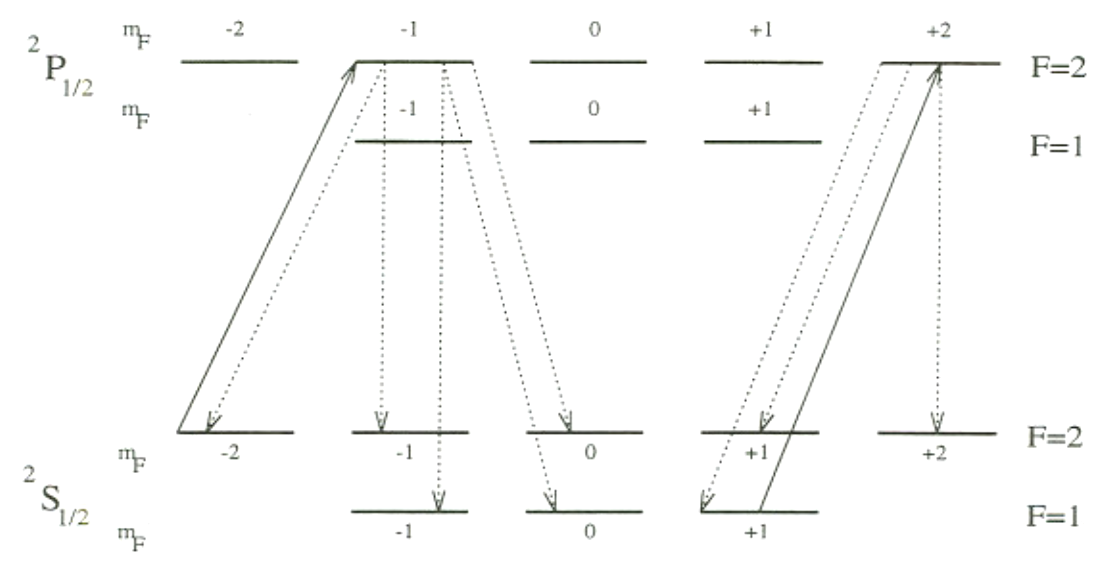
\includegraphics[width=\textwidth]{../img/optPumpen.png}
  \caption{ca.}
\end{center}
\end{figure}
%TODO neues Bild mit Inkscape?

\end{frame}

\subsection{Aufbau}
\begin{frame}
\frametitle{Aufbau: Doppelresonanz}

\setbeamerfont{myfont}{size*=80}
\usebeamerfont{myfont}
\begin{figure}
    \centering
    \def\svgwidth{\textwidth}
    \input{../img/aufbauDR.pdf_tex}
    \caption{Aufbau zur Messung der Doppelresonanz.}
\end{figure}
\usebeamerfont{standard}

\begin{itemize}
  \item \textbf{\textlambda/4-Plättchen:} Erzeugung von zirkular polarisiertem Licht
  \item \textbf{Spule 1:} Einstellbarer Gleichstrom
  \item \textbf{Spule 2:} Sinusförmiger Strom
  \item \textbf{Spule 4:} Kompensation von vertikalem Erdmagnetfeld
  \item \textbf{RF-Sender:} Einstrahlung von elmag. Wechselfeld in die Messzelle
\end{itemize}

\end{frame}



%%% BEN 2.5' %%%

\subsection{Messung}

\begin{frame}
\frametitle{Messung: Doppelresonanz}
\begin{figure}
\begin{center}
  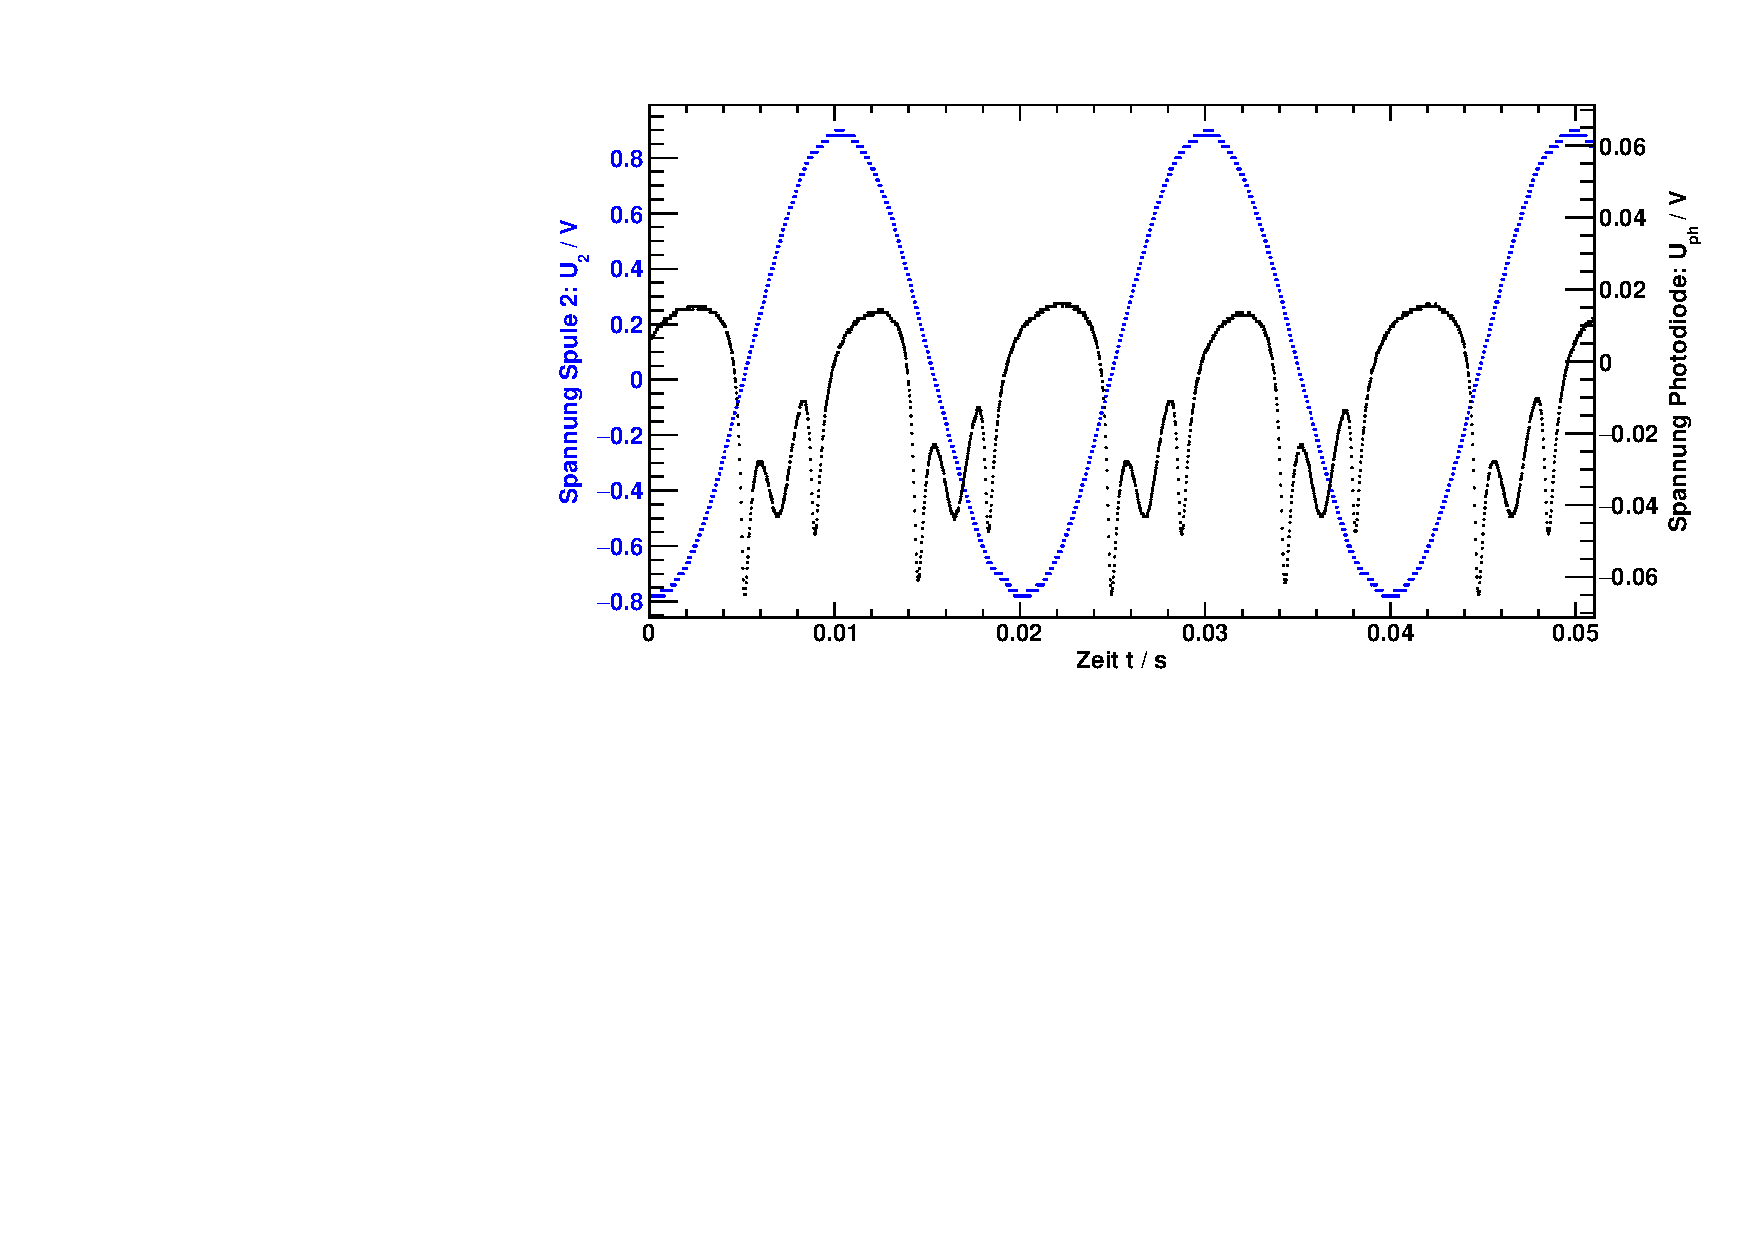
\includegraphics[width=\textwidth]{../img/06.pdf}
  \caption{Starke Modulation des Magnetfelds in Strahlrichtung mit Spule~2 (blau).
   Im Photodiodensignal (schwarz) sind vier Doppelresonanz-Peaks sowie
   zwei Dehmelt-Peaks pro Modulationsperiode sichtbar.}
  \label{img:dehmeltrf}
\end{center}
\end{figure}
\end{frame}

\begin{frame}
\frametitle{Messung: Doppelresonanz}
\begin{figure}
\begin{center}
    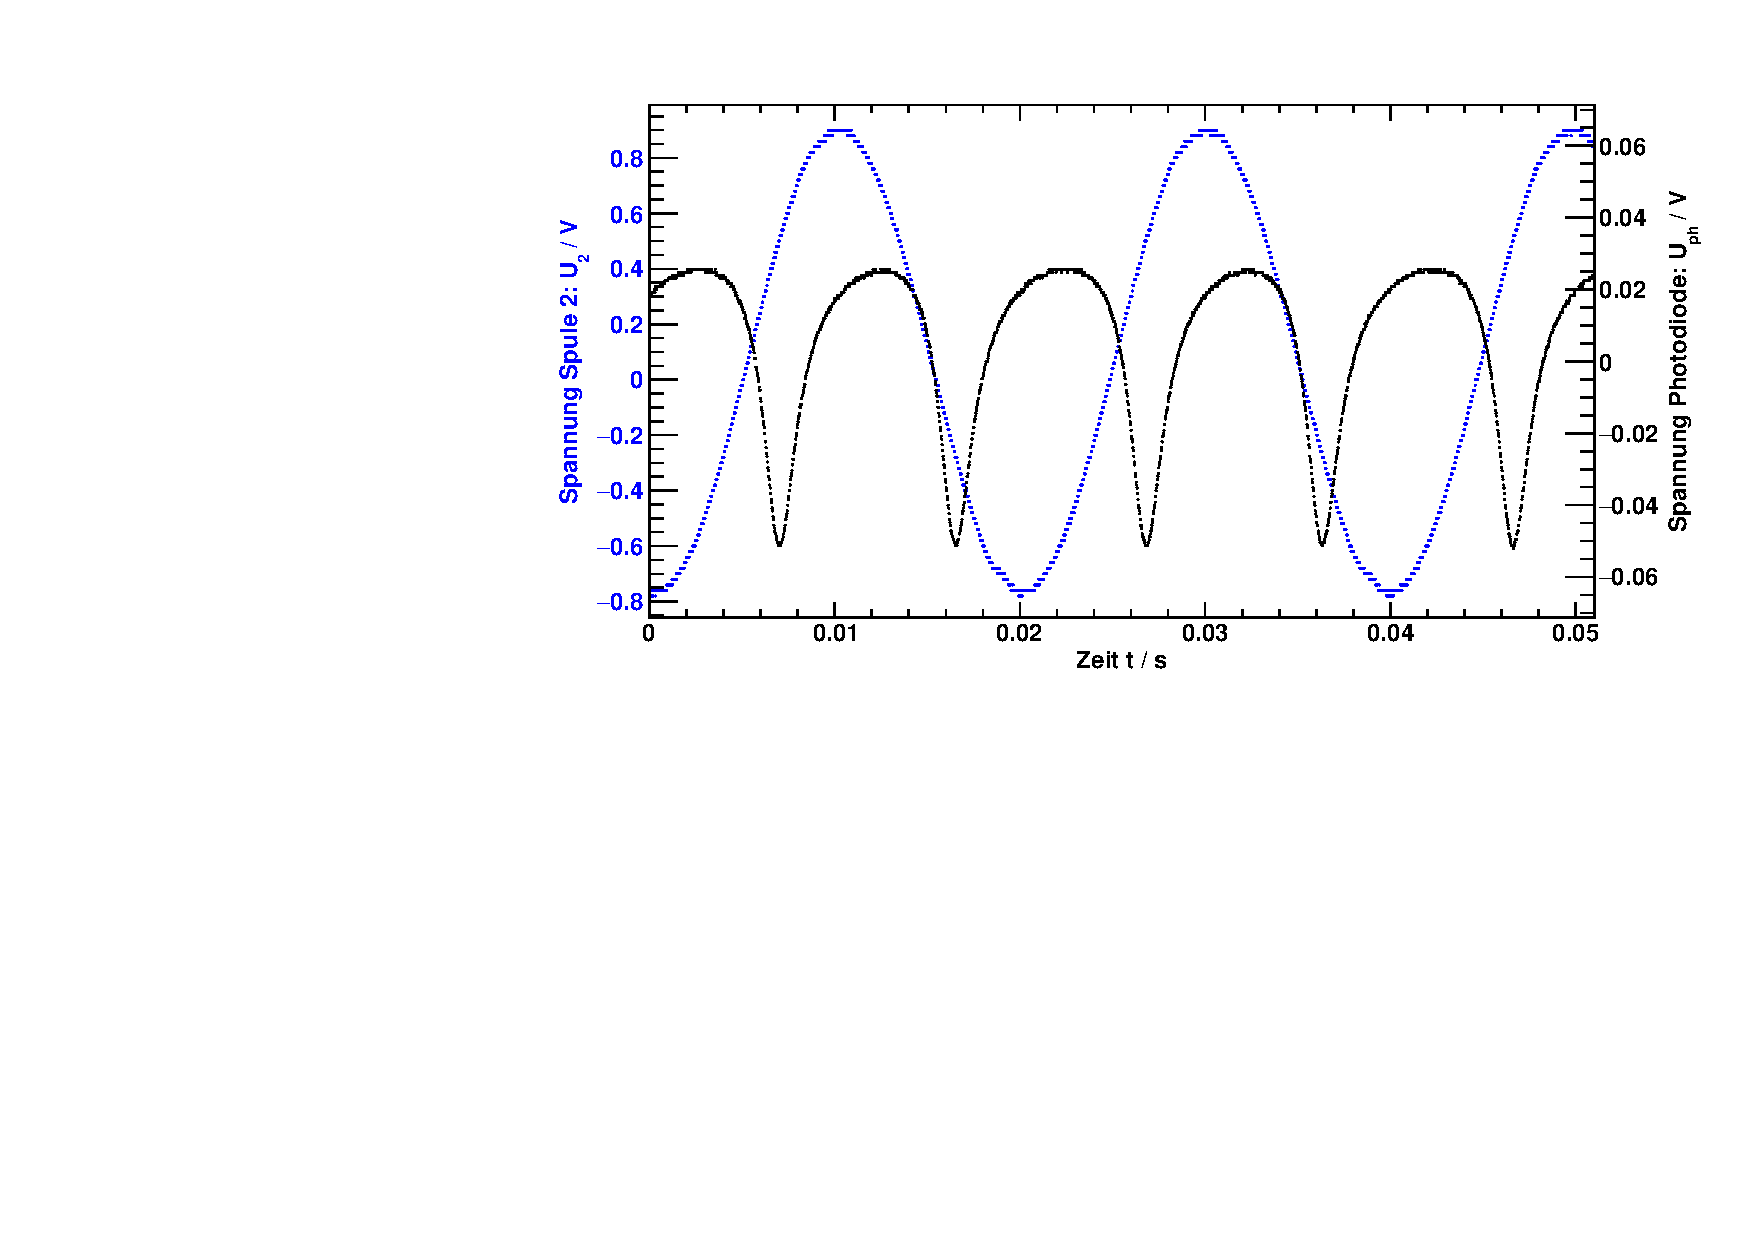
\includegraphics[width=\textwidth]{../img/07.pdf}
    \caption{Gleiches Setup wie bei \autoref{img:dehmeltrf}, aber ohne RF-Signal.
    Die leicht asymmetrischen Dehmelt-Peaks sind weiterhin vorhanden.}
    \label{img:dehmelt}
\end{center}
\end{figure}
\end{frame}

\begin{frame}
\frametitle{Messung: Doppelresonanz}
\begin{figure}
\begin{center}
  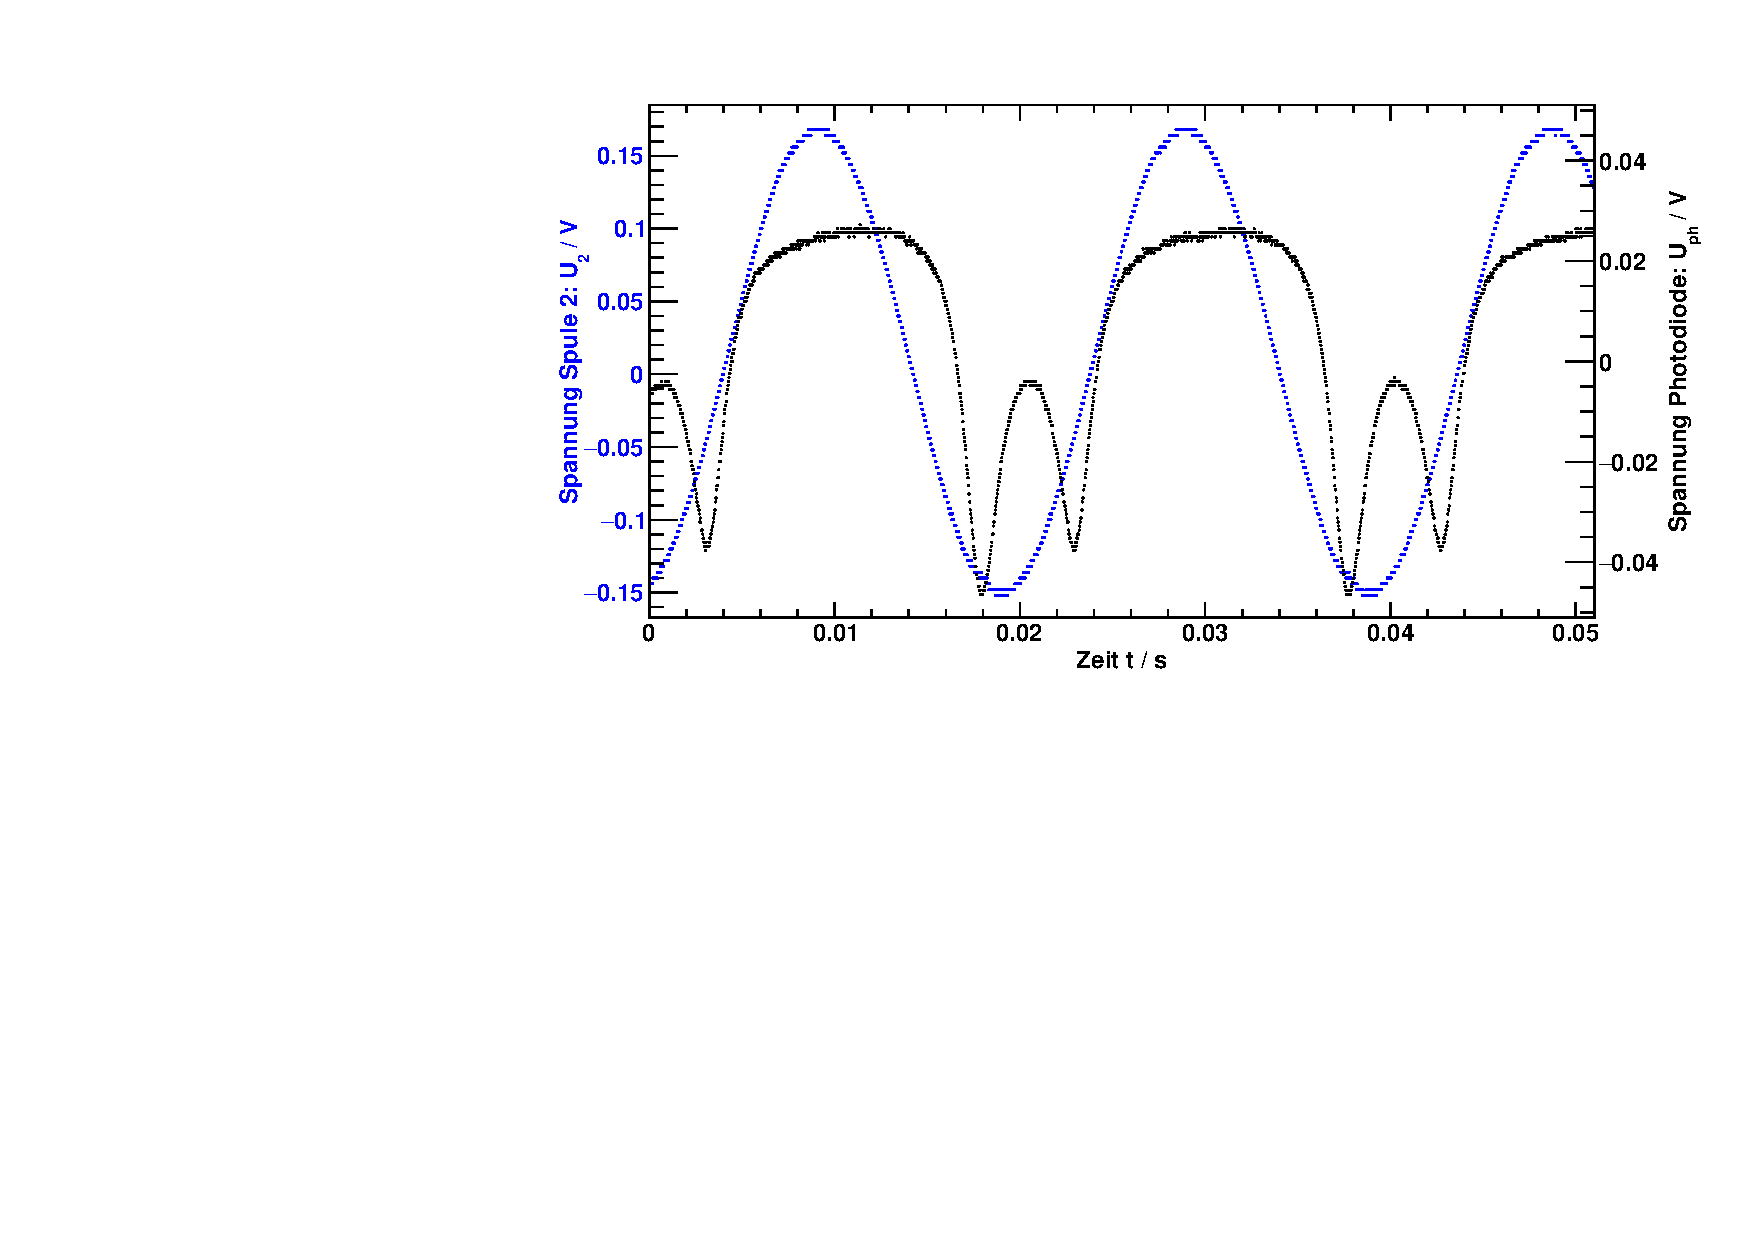
\includegraphics[width=\textwidth]{../img/11.pdf}
  \caption{Doppelresonanz-Absorptionssignal bei kleiner Magnetfeldmodulation:
  Falsche Einstellung des Gleichstroms in Spule~1,
  die Absorptionen sind nicht äquidistant.}
  \label{img:rfwrong}
\end{center}
\end{figure}
\end{frame}

\begin{frame}
\frametitle{Messung: Doppelresonanz}
\begin{figure}
\begin{center}
  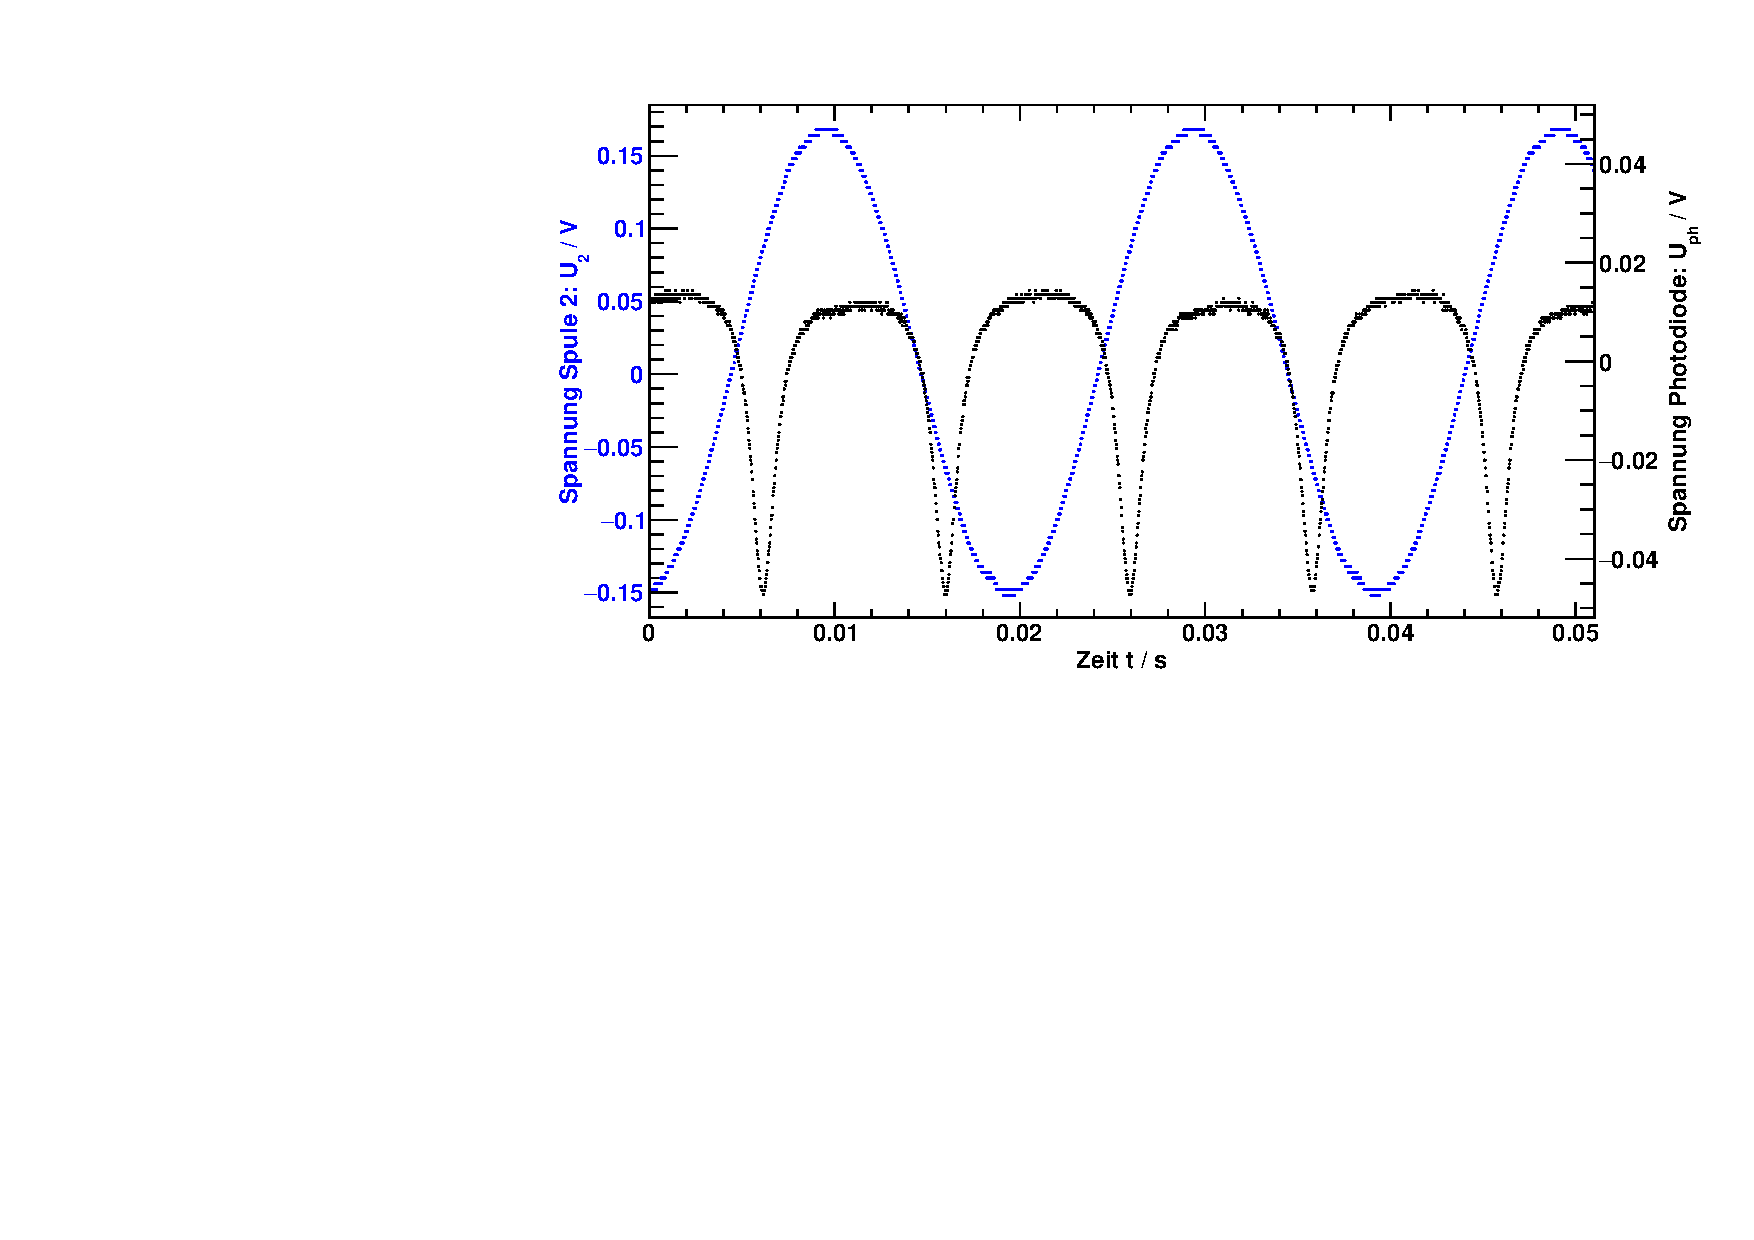
\includegraphics[width=\textwidth]{../img/08.pdf}
  \caption{Doppelresonanz-Absorptionssignal bei kleiner Magnetfeldmodulation:
  Korrekte Einstellung des Gleichstroms in Spule~1,
  die Absorptionen sind daher äquidistant.}
  \label{img:rfcorrect}
\end{center}
\end{figure}
\end{frame}

\subsection{Auswertung}
\begin{frame}
\frametitle{Auswertung: Doppelresonanz}
\begin{itemize}[<+->]
    \item Umrechnung Spulenstrom $\leftrightarrow$ Magnetfeld
    \item Horizontales Magnetfeld
    \begin{equation*}
        B_\text{hor} = \frac{1}{2} \abs{B_1 - B_1'}
    \end{equation*}
    \item Vertikales Magnetfeld
    \begin{equation*}
        B_\text{ver} = B_4
    \end{equation*}
    \item Magnetfeld zur Berechnung des Kernspins $I$
    \begin{equation*}
        \begin{split}
            B_I &= \frac{B_1 + B_1'}{2} \\
            \Rightarrow I &= \frac{\mu_B \cdot B_I}{h \cdot \nu} - \frac{1}{2}
        \end{split}
    \end{equation*}
\end{itemize}
\end{frame}

\begin{frame}
\frametitle{Ergebnisse: Doppelresonanz}
\begin{table}
    \caption{Berechnete horizontale Komponenten des Erdmagnetfeldes und Kernspin von Rubidium für das Doppelresonanzexperiment bei verschiedenen Lasterströmen $I_\text{L}$ und RF-Sender-Frequenzen $\nu$.}
    \begin{center}
        \begin{tabular}{|c|c|c|c|c|}
            \hline
            $I_\text{L}$ / mA & $\nu$ / kHz & $B_\text{hor}$ / \textmu T & $I$ \\ \hline
            62.9 & 493.98 & $12.4 \pm 1.1$ & $2.50 \pm 0.03$ \\ \hline
            62.9 & 899.41 & $12.8 \pm 2.3$ & $2.53 \pm 0.04$ \\ \hline
            63.2 & 493.77 & $12.0 \pm 1.1$ & $1.52 \pm 0.03$ \\ \hline
            63.2 & 899.67 & $12.4 \pm 1.1$ & $1.53 \pm 0.02$ \\ \hhline{|==|=|=|}
            \multicolumn{2}{|c|}{gew. Mittel \rb{85}} & \multirow{2}{*}{$12.3 \pm 0.6$} & $2.51 \pm 0.02$ \\ \cline{1-2} \cline{4-4}
            \multicolumn{2}{|c|}{gew. Mittel \rb{87}} & & $1.527 \pm 0.016$ \\ \hline
            \multicolumn{2}{|c|}{Lit./theo. Wert \rb{85}} & \multirow{2}{*}{$20.9$} & 2.5 \\ \cline{1-2} \cline{4-4}
            \multicolumn{2}{|c|}{Lit./theo. Wert \rb{87}} & & 1.5 \\ \hline
        \end{tabular}
    \end{center}
\end{table}
\begin{equation*}
    \begin{split}
       & B_\text{ver} = (40.94 \pm 1.43)\,\text{\textmu T} \\
       & B_\text{ver}^{\text{Lit.}} = 42.9\,\text{\textmu T}
    \end{split}    
\end{equation*}
\end{frame}
%%% MORITZ 10' %%%

\section{Spinpräzession}
\subsection{Grundlagen}
\begin{frame}
\frametitle{Grundlagen: Spinpräzession}

\begin{itemize}
  \item Spinpräzession von Atomen im Magnetfeld $B$ mit Frequenz $f$
\end{itemize}


\begin{equation*}
    f=\frac{g_\text{F} \cdot \mu_\text{B}}{h} \cdot B = \alpha \cdot B
\end{equation*}
  
  
\begin{equation*}
    \alpha = 4.665\,\text{kHz } \text{\textmu T}^{-1}
\end{equation*}

\end{frame}

\subsection{Aufbau}
\begin{frame}
\frametitle{Aufbau: Spinpräzession}

\setbeamerfont{myfont}{size*=80}
\usebeamerfont{myfont}
\begin{figure}
    \centering
    \def\svgwidth{\textwidth}
    \input{../img/aufbauspinpraez.pdf_tex}
    \caption{Aufbau zur Messung der Spinpräzession.}
\end{figure}
\usebeamerfont{standard}

\begin{itemize}
  \item \textbf{Spule 1:} Kompensation von horizontalem Erdmagnetfeld
  \item \textbf{Spule 4:} Kompensation von vertikalem Erdmagnetfeld
  \item \textbf{Spule 5:} Ein- und Ausschalten von Magnetfeld mit 50\,Hz
\end{itemize}

\end{frame}

\subsection{Auswertung}

\begin{frame}
\frametitle{Auswertung: Spinpräzession}

\begin{figure}
    \centering
    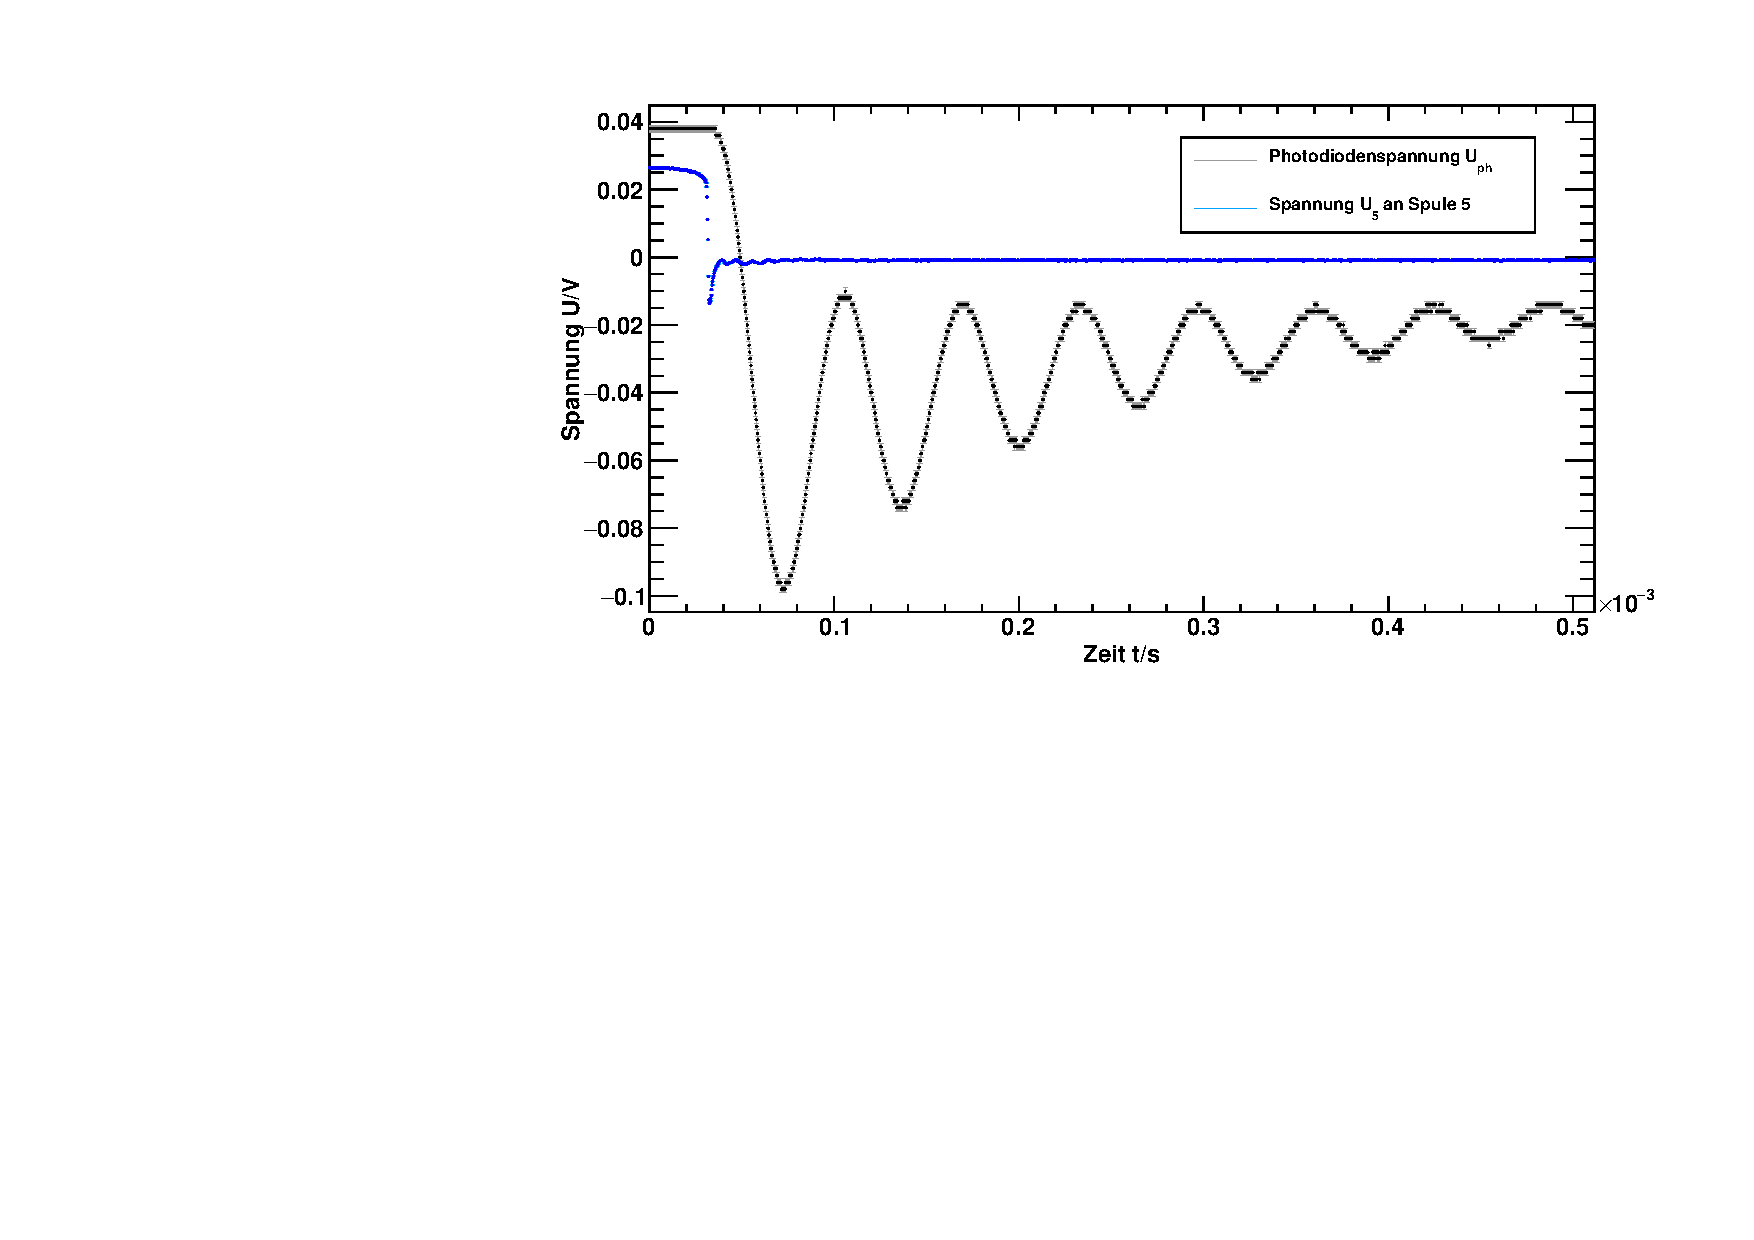
\includegraphics[width=\textwidth]{../img/02-63-7mA-087mA.pdf}
    \caption{Spinpräzession im schwachen Magnetfeld.}  
\end{figure} 
  
\end{frame}


\begin{frame}
\frametitle{Auswertung: Spinpräzession}

\begin{figure}
    \centering
    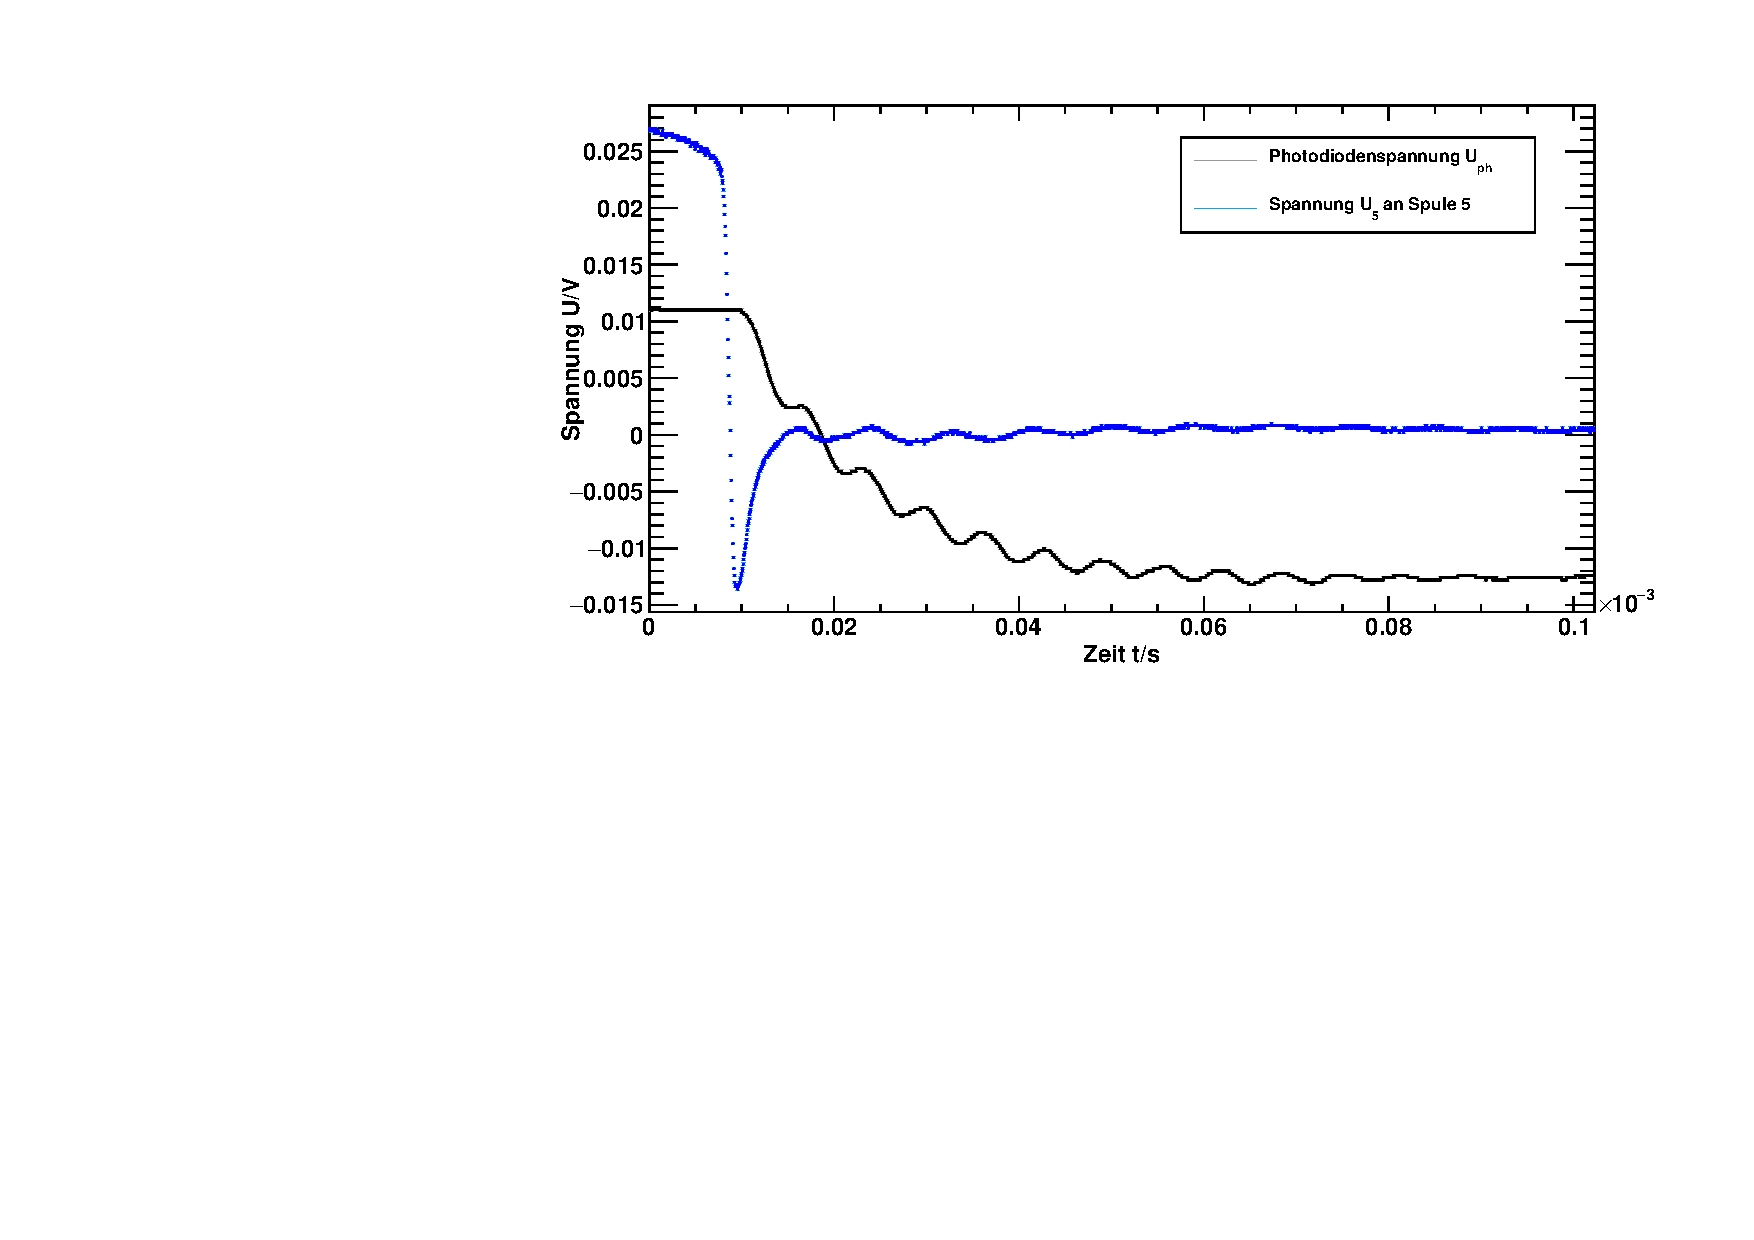
\includegraphics[width=\textwidth]{../img/02-63-7mA-020mA.pdf}
    \caption{Spinpräzession im starken Magnetfeld.}  
\end{figure} 
  
\end{frame}



\begin{frame}
\frametitle{Auswertung: Spinpräzession}

\begin{figure}
    \centering
    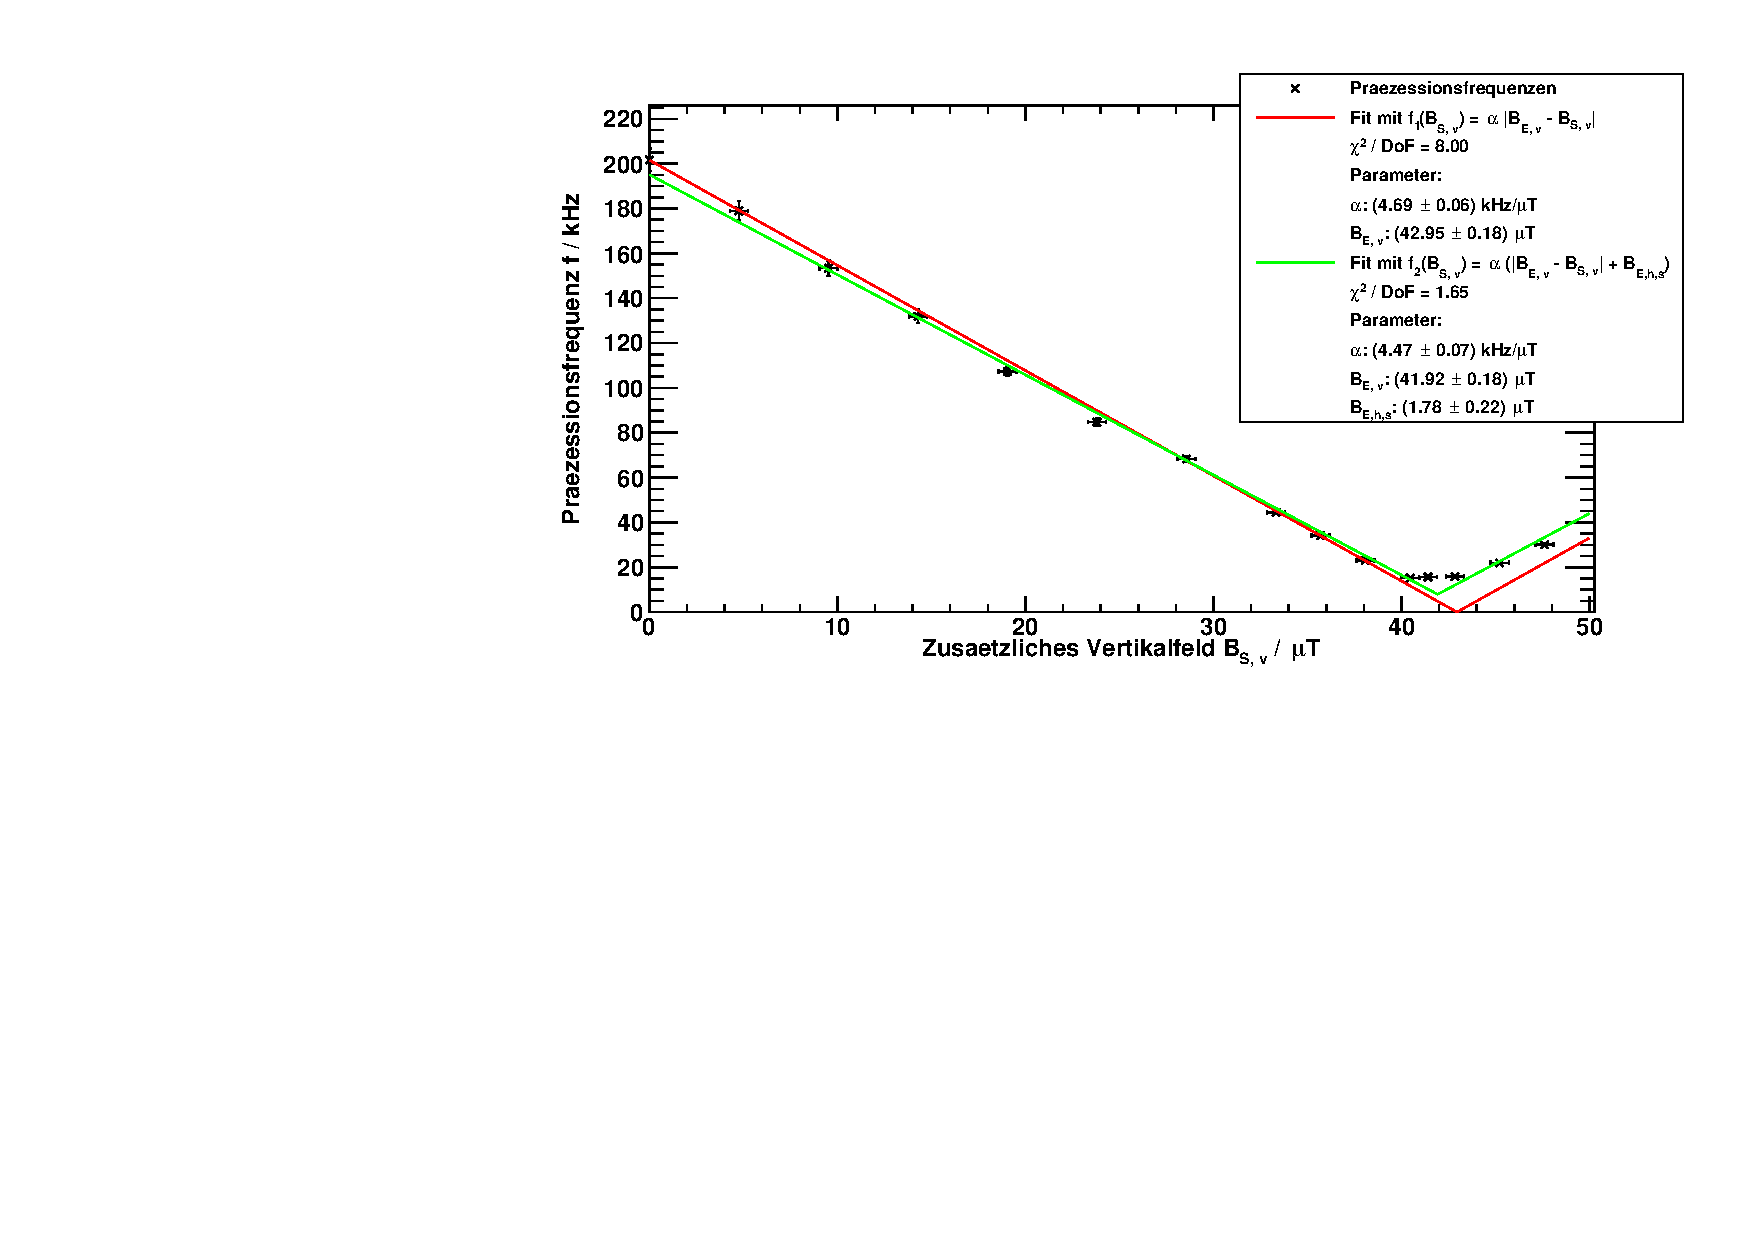
\includegraphics[width=\textwidth]{../img/Rb85.pdf}
    \caption{Magnetfeldabhängigkeit der Spinpräzessionsfrequenz.}  
\end{figure} 
  
\end{frame}


\begin{frame}
\frametitle{Auswertung: Spinpräzession}

Horizontalkomponente des Erdmagnetfelds war nicht vollständig kompensierbar
$\to$ Berechnung der Winkelabweichung des Messaufbaus von der Nordrichtung
\begin{equation*}
    \varphi = \arctan\left( \frac{B_\text{h,s}}{B_\text{h,p}} \right)
    = (8.3 \pm 1.0)^\circ
\end{equation*}

\setbeamerfont{myfont}{size*=80}
\usebeamerfont{myfont}
\begin{figure}
    \centering
    \def\svgwidth{0.5\textwidth}
    \input{../img/arctangans.pdf_tex}
    \caption{Horizontalkomponenten des Erdmagnetfelds senkrecht und parallel zur Strahlrichtung.}
\end{figure}
\usebeamerfont{standard}
  
\end{frame}

\begin{frame}
\frametitle{Auswertung: Spinpräzession}

\begin{figure}
    \centering
    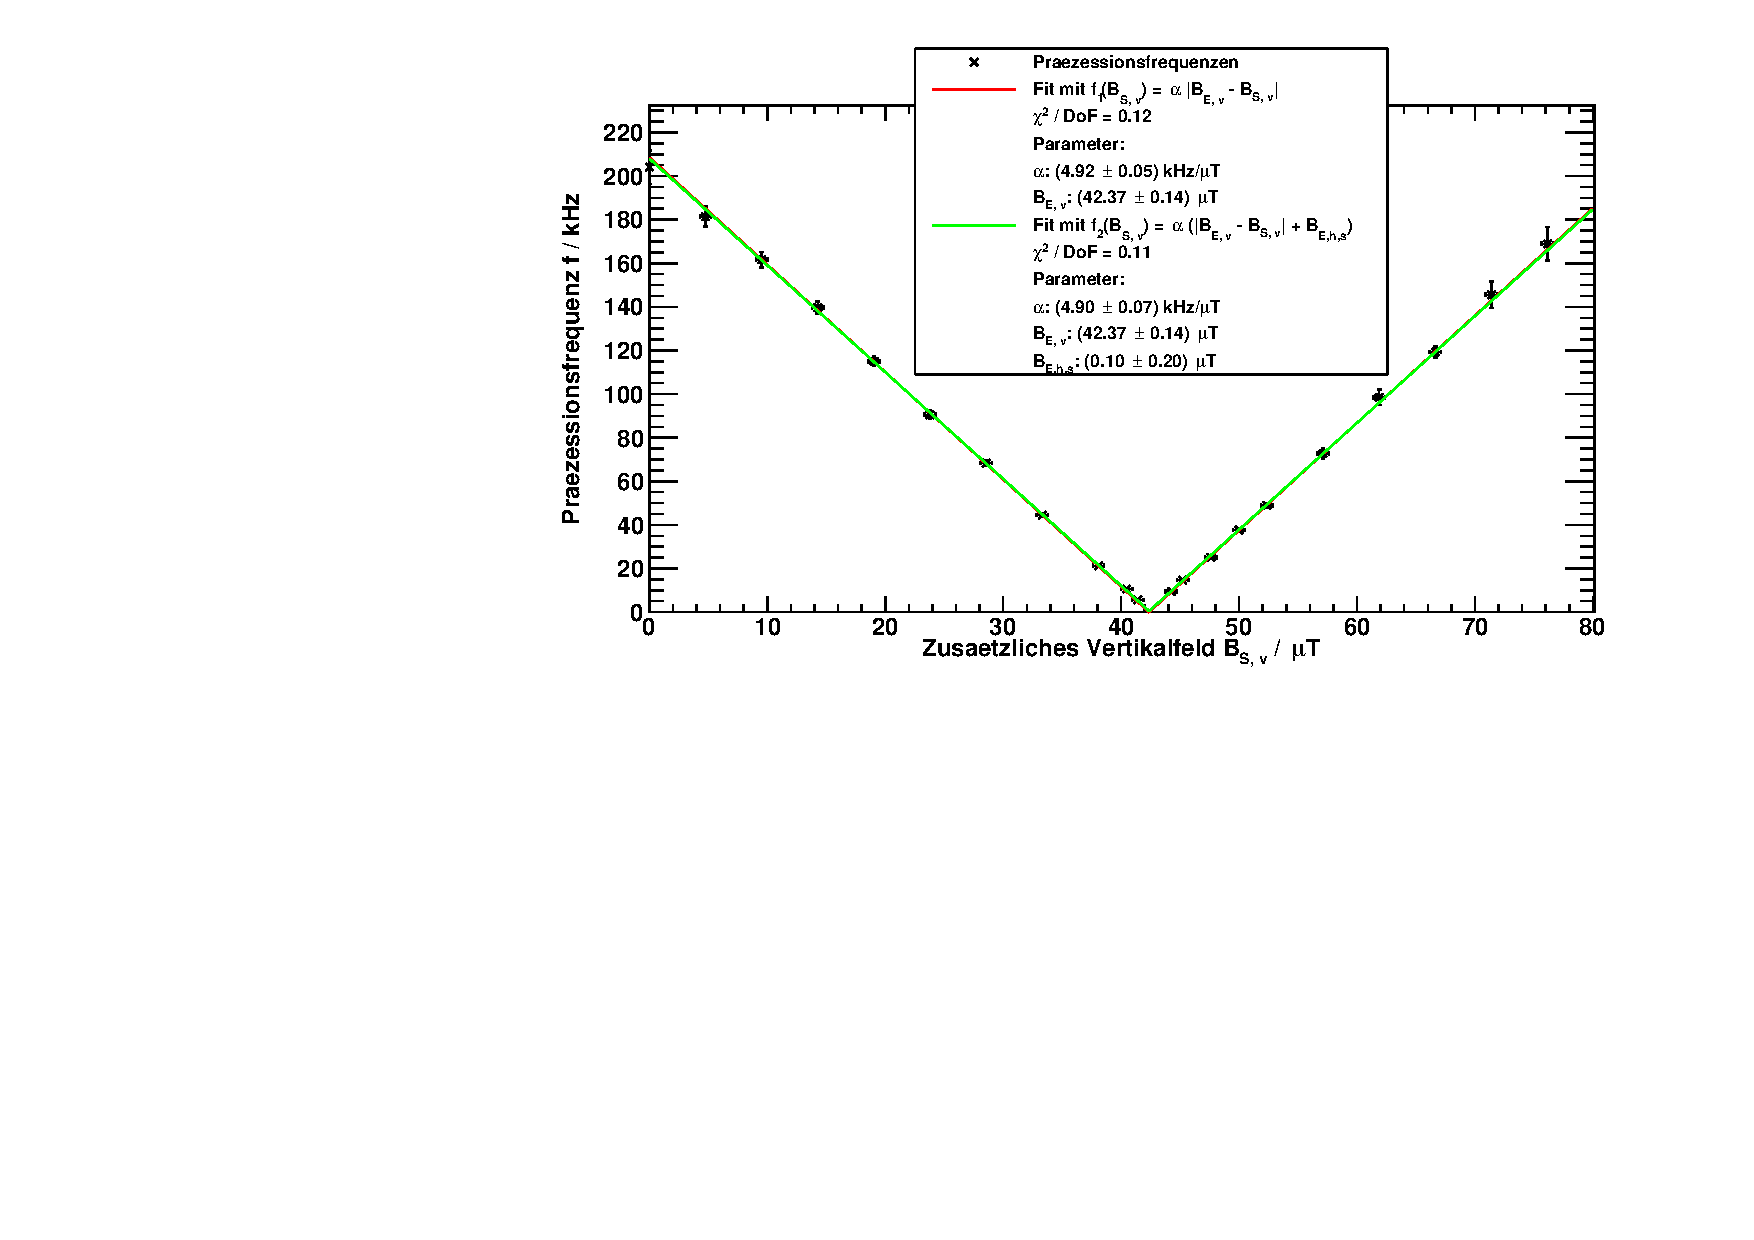
\includegraphics[width=\textwidth]{../img/Rb85_gedreht.pdf}
    \caption{Magnetfeldabhängigkeit der Spinpräzessionsfrequenz nach Ausrichtung des Versuchsaufbaus nach Norden.}  
\end{figure} 
  
\end{frame}




\begin{frame}
\frametitle{Auswertung: Spinpräzession}

\begin{figure}
    \centering
    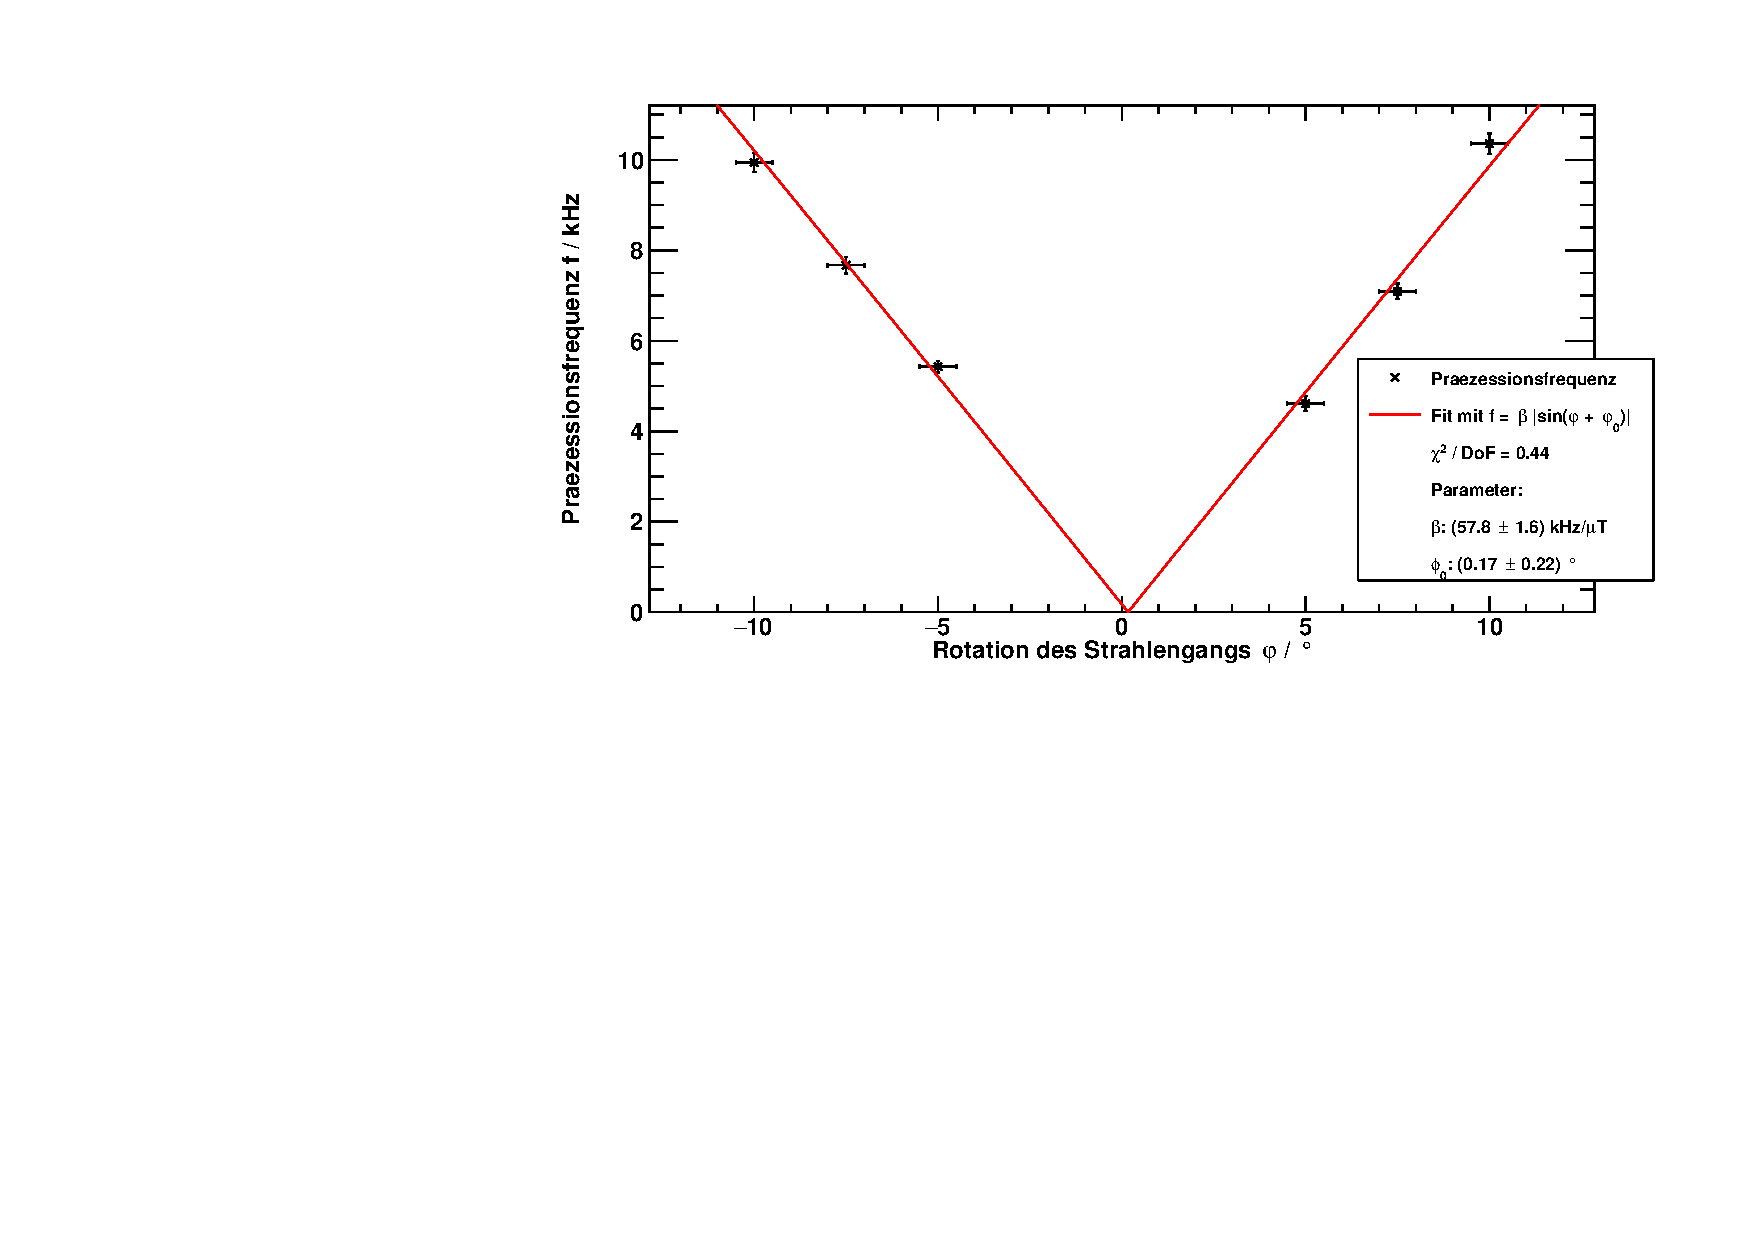
\includegraphics[width=\textwidth]{../img/winkel.pdf}
    \caption{Winkelabhängigkeit der Spinpräzessionsfrequenz.}  
\end{figure} 
  
\end{frame}

\begin{frame}
\frametitle{Ergebnis: Spinpräzession}
\begin{itemize}
    \item Zusammenhang zwischen Magnetfeld und Frequenz
    \begin{equation*}
        \alpha^\text{exp} = 4.92 \pm 0.05\,\text{kHz } \text{\textmu T}^{-1}
    \end{equation*}
    \item Literaturwert
    \begin{equation*}
        \alpha^\text{theo} = 4.665\,\text{kHz } \text{\textmu T}^{-1}
    \end{equation*}
    \item Abweichung durch Umrechnung von Spulenstrom in Magnetfeldstärke?
\end{itemize}
  
\end{frame}

%%% BEN 5' %%%

\section{Bestimmung der Relaxationszeit nach Dehmelt}
\subsection{Grundlagen: Relaxationsprozesse}

\begin{frame}
\frametitle{Grundlagen: Relaxationsprozesse beim optischen Pumpen}
\begin{itemize}[<+->]
    \item Pumpzeit $T_\text{P}$
    \begin{equation*}
        \left(\frac{\difd n}{\difd t}\right)_{\text{Pump}}=\frac{N-n}{T_\text{P}}
    \end{equation*}
    $N$: Anzahl der Atome in Ensemble, $n$: Differenz der Besetzungszahlen
    \item Relaxation durch
    \begin{itemize}[<+->]
        \item Wechselwirkung mit Wand der Messzelle
        \item Stöße mit dem Puffergas
        \item Spinaustausch zwischen Rubidiumatomen
    \end{itemize}
    \item Relaxationszeit $T_\text{R}$
    \begin{equation*}
        \left(\frac{\difd n}{\difd t}\right)_{\text{Relax}}=-\frac{n}{T_\text{R}}
    \end{equation*}
\end{itemize}
\end{frame}

\begin{frame}
\frametitle{Grundlagen: Relaxationsprozesse beim optischen Pumpen}
\begin{itemize}[<+->]
    \item Orientierungsprozess
    \begin{equation*}
        \left(\frac{\difd n}{\difd t}\right)_{\text{Orient}}
        =\left(\frac{\difd n}{\difd t}\right)_{\text{Pump}} + \left(\frac{\difd n}{\difd t}\right)_{\text{Relax}}
        =\frac{N}{T_\text{P}}-n \left( \frac{1}{T_\text{P}} + \frac{1}{T_\text{R}}\right)
    \end{equation*}
    \item Orientierungszeit $\tau$
    \begin{equation*}
        \begin{split}
            \left(\frac{\difd n}{\difd t}\right)_{\text{Orient}} &= \frac{N}{T_\text{P}}- \frac{n}{\tau} \quad \Rightarrow \quad n(t) \sim e^{-\frac{t}{\tau}} \\
            \frac{1}{\tau} :&= \frac{1}{T_\text{P}} + \frac{1}{T_\text{R}}
        \end{split}
    \end{equation*}
    \item Pumpzeit $T_\text{P}$ ist umgekehrt proportional zur Intensität $I$
    \begin{equation*}
        \frac{1}{T_\text{P}} = \alpha I
    \end{equation*}
\end{itemize}
\end{frame}



\subsection{Aufbau}
\begin{frame}
\frametitle{Aufbau: Bestimmung der Relaxationszeit nach Dehmelt}

\setbeamerfont{myfont}{size*=80}
\usebeamerfont{myfont}
\begin{figure}
    \centering
    \def\svgwidth{\textwidth}
    \input{../img/aufbaudehmelt.pdf_tex}
    \caption{Aufbau zur Bestimmung der Relaxationszeit nach Dehmelt.}
\end{figure}
\usebeamerfont{standard}

\begin{itemize}
    \item \textbf{ND-Filter:} Abschwächung der Laserintensität um 60\% bis 98\%
    \item \textbf{Spule 3:} Rechteckiges Wechselfeld mit 50\,Hz
    \item \textbf{Spule 4:} Kompensation von vertikalem Erdmagnetfeld
\end{itemize}
\end{frame}

\begin{frame}
\frametitle{Optisches Pumpen}
\setbeamerfont{myfont}{size*=80}
\usebeamerfont{myfont}
\begin{figure}
    \centering
    \def\svgwidth{\textwidth}
    \input{../img/optPumpen.pdf_tex}
    \caption{Zeeman-Pumpen von \rb{85} mit \textsigma$^+$-Licht.}
\end{figure}
\end{frame}

\subsection{Auswertung}
\begin{frame}
\frametitle{Auswertung: Bestimmung der Orientierungszeit}
\begin{figure}
    \begin{center}
        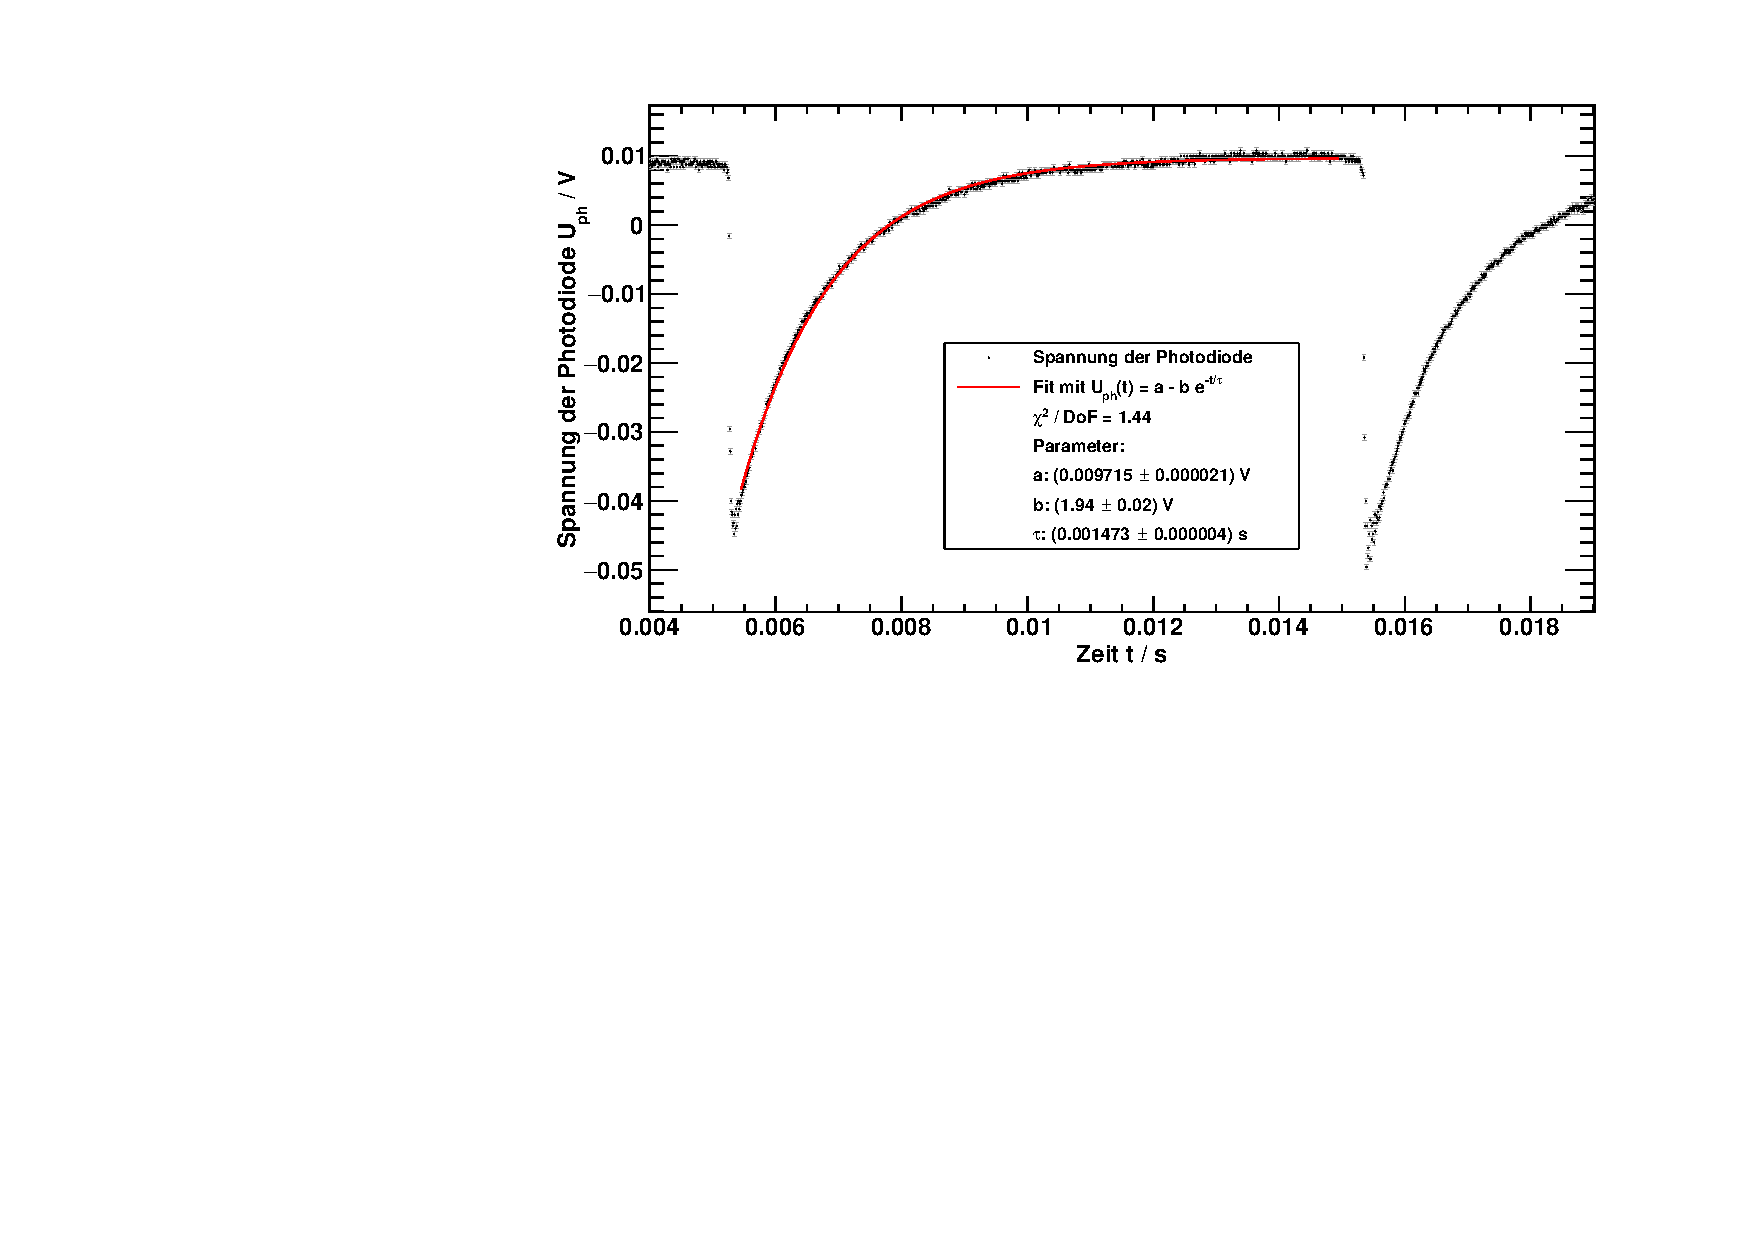
\includegraphics[width=\textwidth]{../img/65-5mA-10.pdf}
        \caption{Transmission nach Umpolung des horizontalen Magnetfeldes.}
    \end{center}
\end{figure}
\end{frame}

\begin{frame}
\frametitle{Auswertung: Bestimmung der Orientierungszeit}
\begin{itemize}[<+->]
    \item Fit mit
    \begin{equation*}
        U_{\text{ph}}(t)=a - b \cdot e^{-\frac{t}{\tau}}
    \end{equation*}
    für verschiedene Intensitäten
    \item Fit der Orientierungszeiten $\tau(I)$ 
    \begin{equation*}
        \frac{1}{\tau(I)}=\alpha I + \frac{1}{T_{\text{R}_\text{D}}}
    \end{equation*}
\end{itemize}
\end{frame}

\begin{frame}
\frametitle{Auswertung: Extrapolation auf keine Intensität}
\begin{figure}
    \begin{center}
        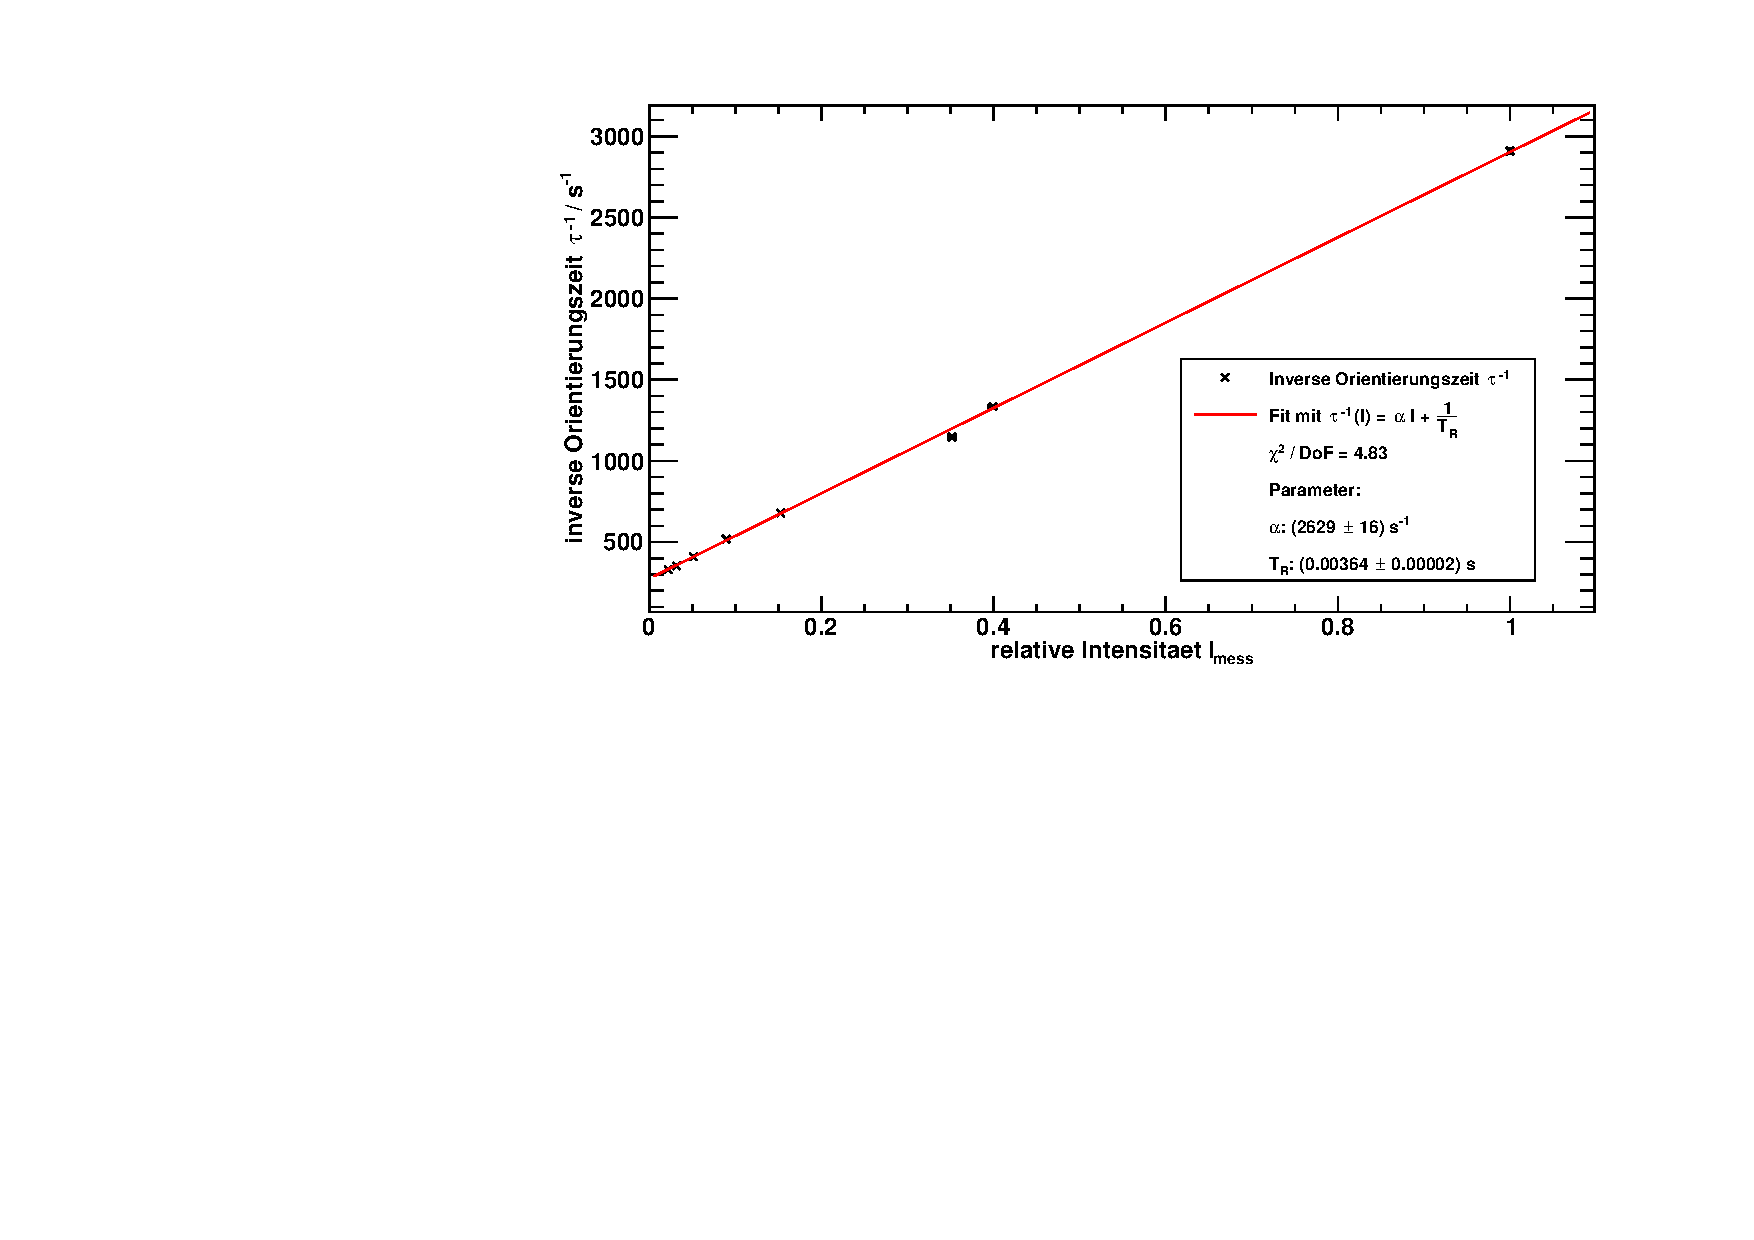
\includegraphics[width=\textwidth]{../img/taufit.pdf}
        \caption{Bestimmung der Relaxationszeit $T_{\text{R}_\text{D}}$ mit Achsenabschnitt.}
    \end{center}
\end{figure}
\end{frame}

\begin{frame}
\frametitle{Ergebnis: Bestimmung der Relaxationszeit nach Dehmelt}
\begin{itemize}[<+->]
    \item Relaxationszeit
    \begin{equation*}
        T_{\text{R}_\text{D}} = 3.64 \pm 0.02\,\text{ms}
    \end{equation*}
    \item Literaturwert
    \begin{equation*}
        T_{\text{R}}^\text{Lit.} = 6.5\,\text{ms}
    \end{equation*}
    \item Mögliche Fehlerquelle: Andere Relaxationsmechanismen
\end{itemize}
\end{frame}
%%% MORITZ 5' %%%

\section{Bestimmung der Relaxationszeit nach Franzen}
\subsection{Grundlagen}

\begin{frame}
\frametitle{Grundlagen: Bestimmung der Relaxationszeit nach Franzen}

\setbeamerfont{myfont}{size*=80}
\usebeamerfont{myfont}
\begin{figure}
    \centering
    \def\svgwidth{\textwidth}
    \input{../img/FranzenTheo0.pdf_tex}
    \caption{Theoretischer Verlauf der Polarisation/Transmission bei der Messmethode nach Franzen.}
\end{figure}

  
\end{frame}


\begin{frame}[noframenumbering]
\frametitle{Grundlagen: Bestimmung der Relaxationszeit nach Franzen}

\setbeamerfont{myfont}{size*=80}
\usebeamerfont{myfont}
\addtocounter{figure}{-1}
\begin{figure}
    \centering
    \def\svgwidth{\textwidth}
    \input{../img/FranzenTheo.pdf_tex}
    \caption{Theoretischer Verlauf der Polarisation/Transmission bei der Messmethode nach Franzen.}
\end{figure}

  
\end{frame}

\subsection{Aufbau}
\begin{frame}
\frametitle{Aufbau: Bestimmung der Relaxationszeit nach Franzen}

\setbeamerfont{myfont}{size*=80}
\usebeamerfont{myfont}
\begin{figure}
    \centering
    \def\svgwidth{\textwidth}
    \input{../img/aufbaufranzen.pdf_tex}
    \caption{Aufbau zur Bestimmung der Relaxationszeit nach Franzen.}
\end{figure}
\usebeamerfont{standard}

\begin{itemize}
  \item \textbf{Chopper:} Periodische Unterbrechung des Laserlichts
\end{itemize}

\end{frame}

\subsection{Auswertung}
\begin{frame}
\frametitle{Auswertung: Bestimmung der Relaxationszeit nach Franzen}

\begin{figure}
    \centering
    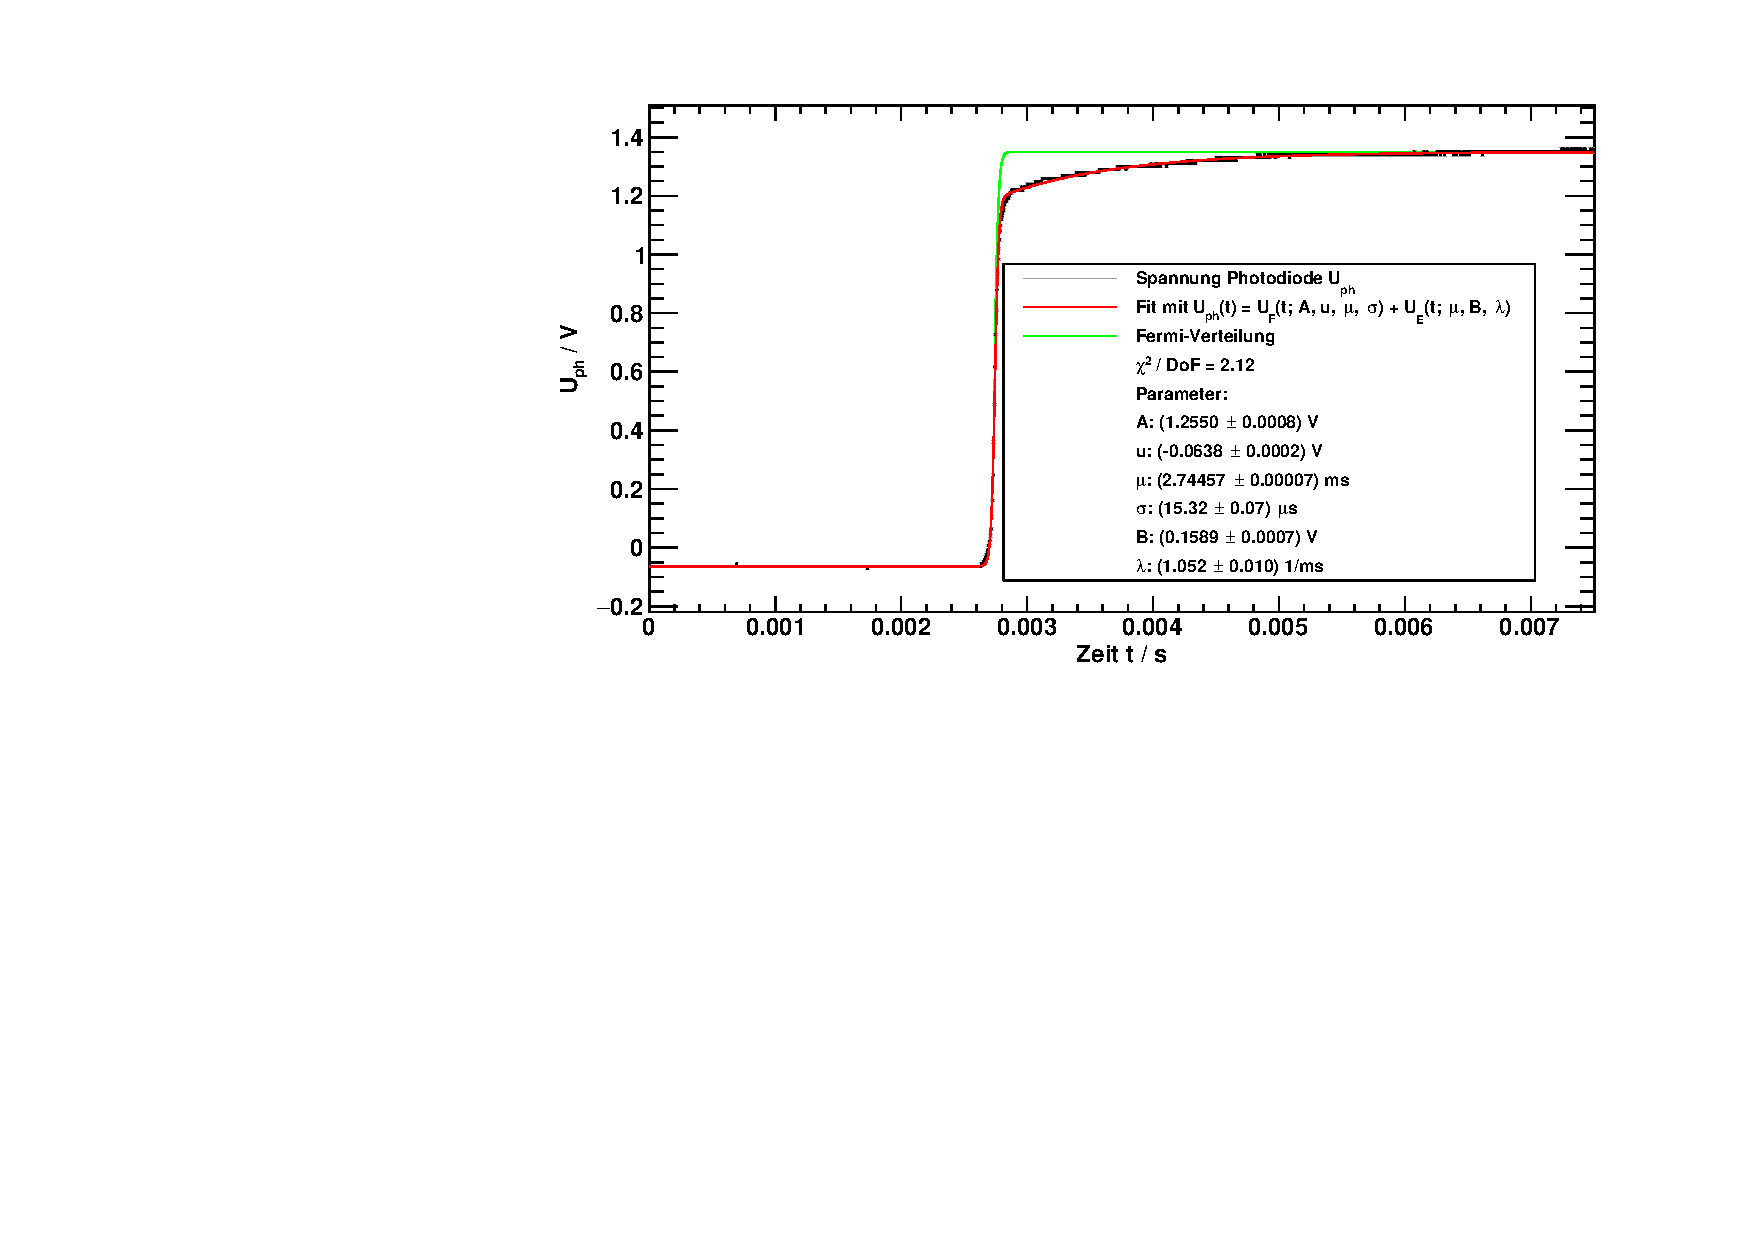
\includegraphics[width=\textwidth]{../img/04.pdf}
    \caption{Transmission der Messzelle nach Öffnung des Strahlengangs.}  
\end{figure} 
  
\end{frame}


\begin{frame}
\frametitle{Auswertung: Bestimmung der Relaxationszeit nach Franzen}

\begin{figure}
    \centering
    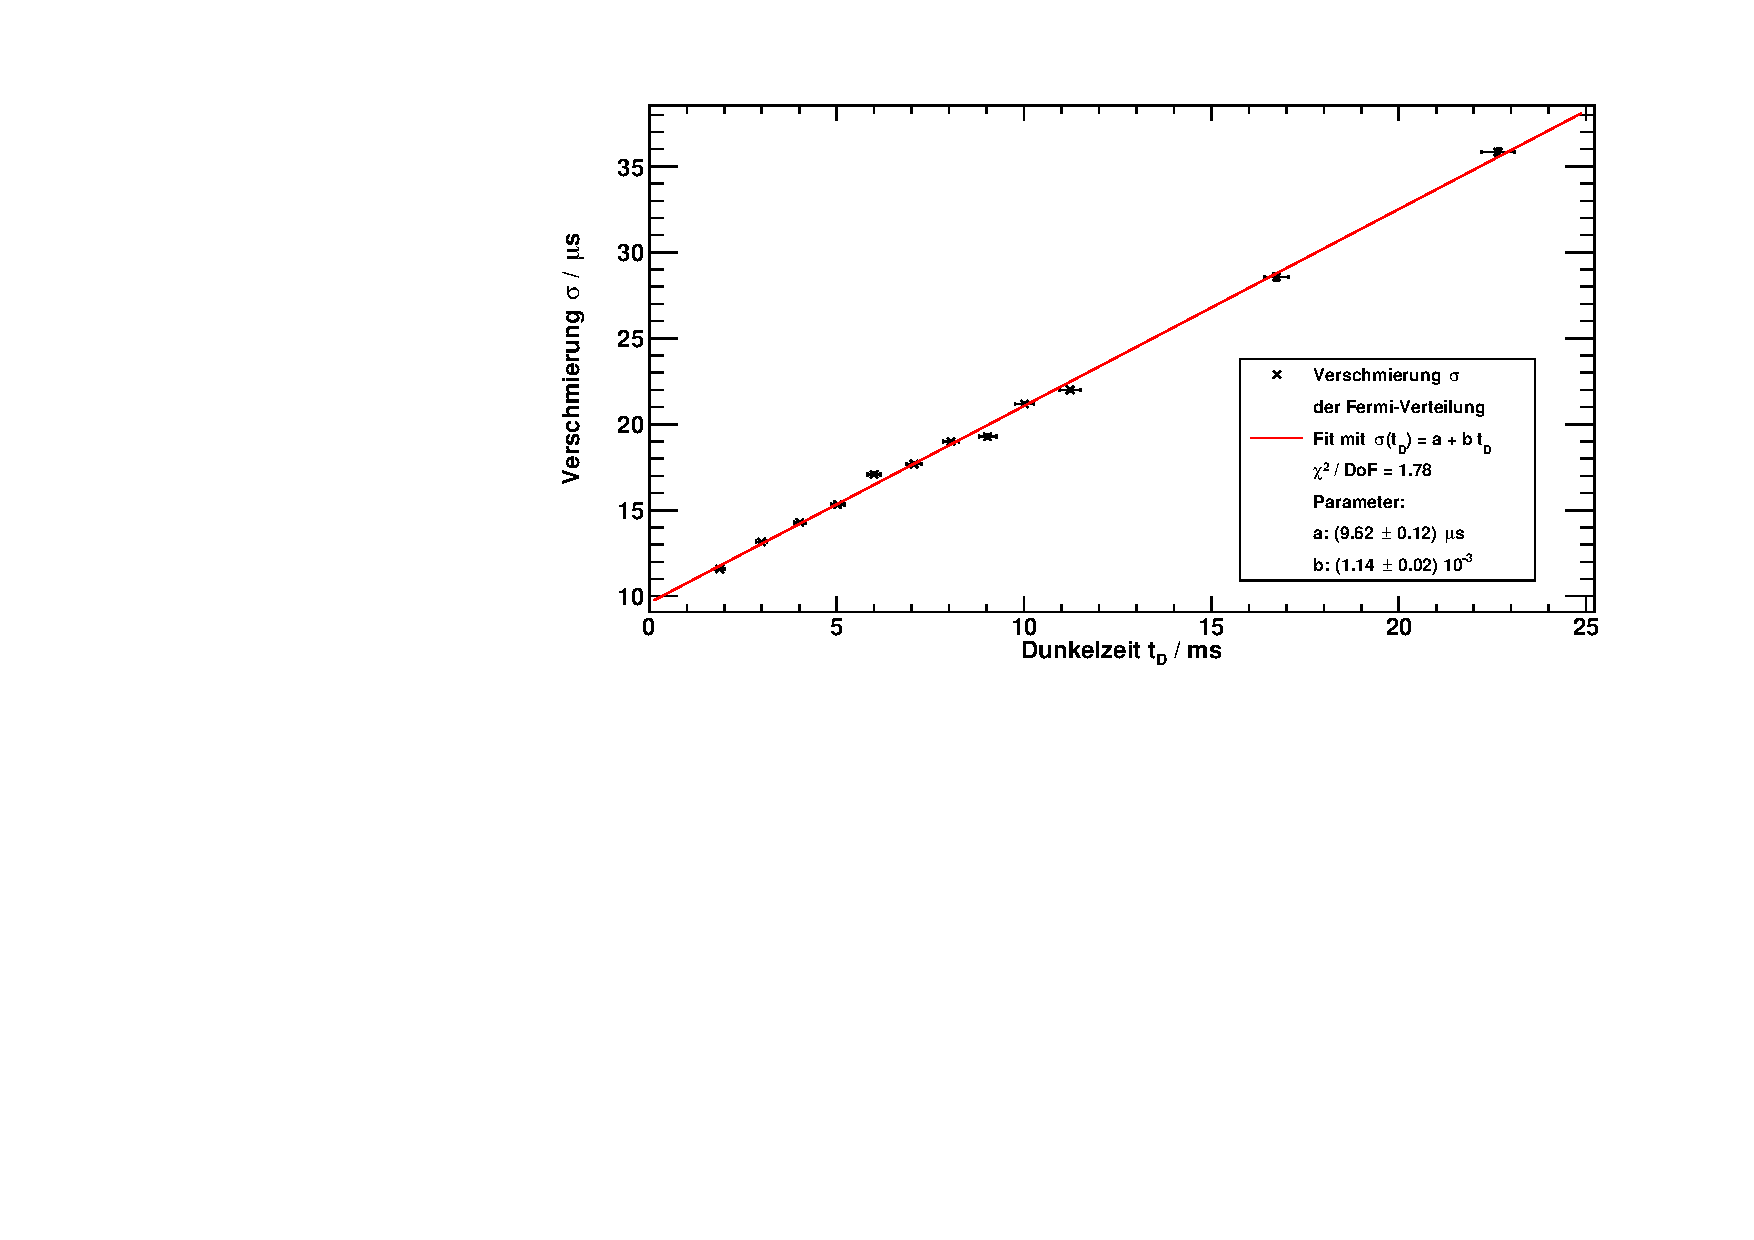
\includegraphics[width=\textwidth]{../img/sigmaFit.pdf}
    \caption{Abrundung $\sigma$ der gefitteten Fermi-Funktionen.}  
\end{figure} 
  
\end{frame}


\begin{frame}
\frametitle{Auswertung: Bestimmung der Relaxationszeit nach Franzen}

\begin{figure}
    \centering
    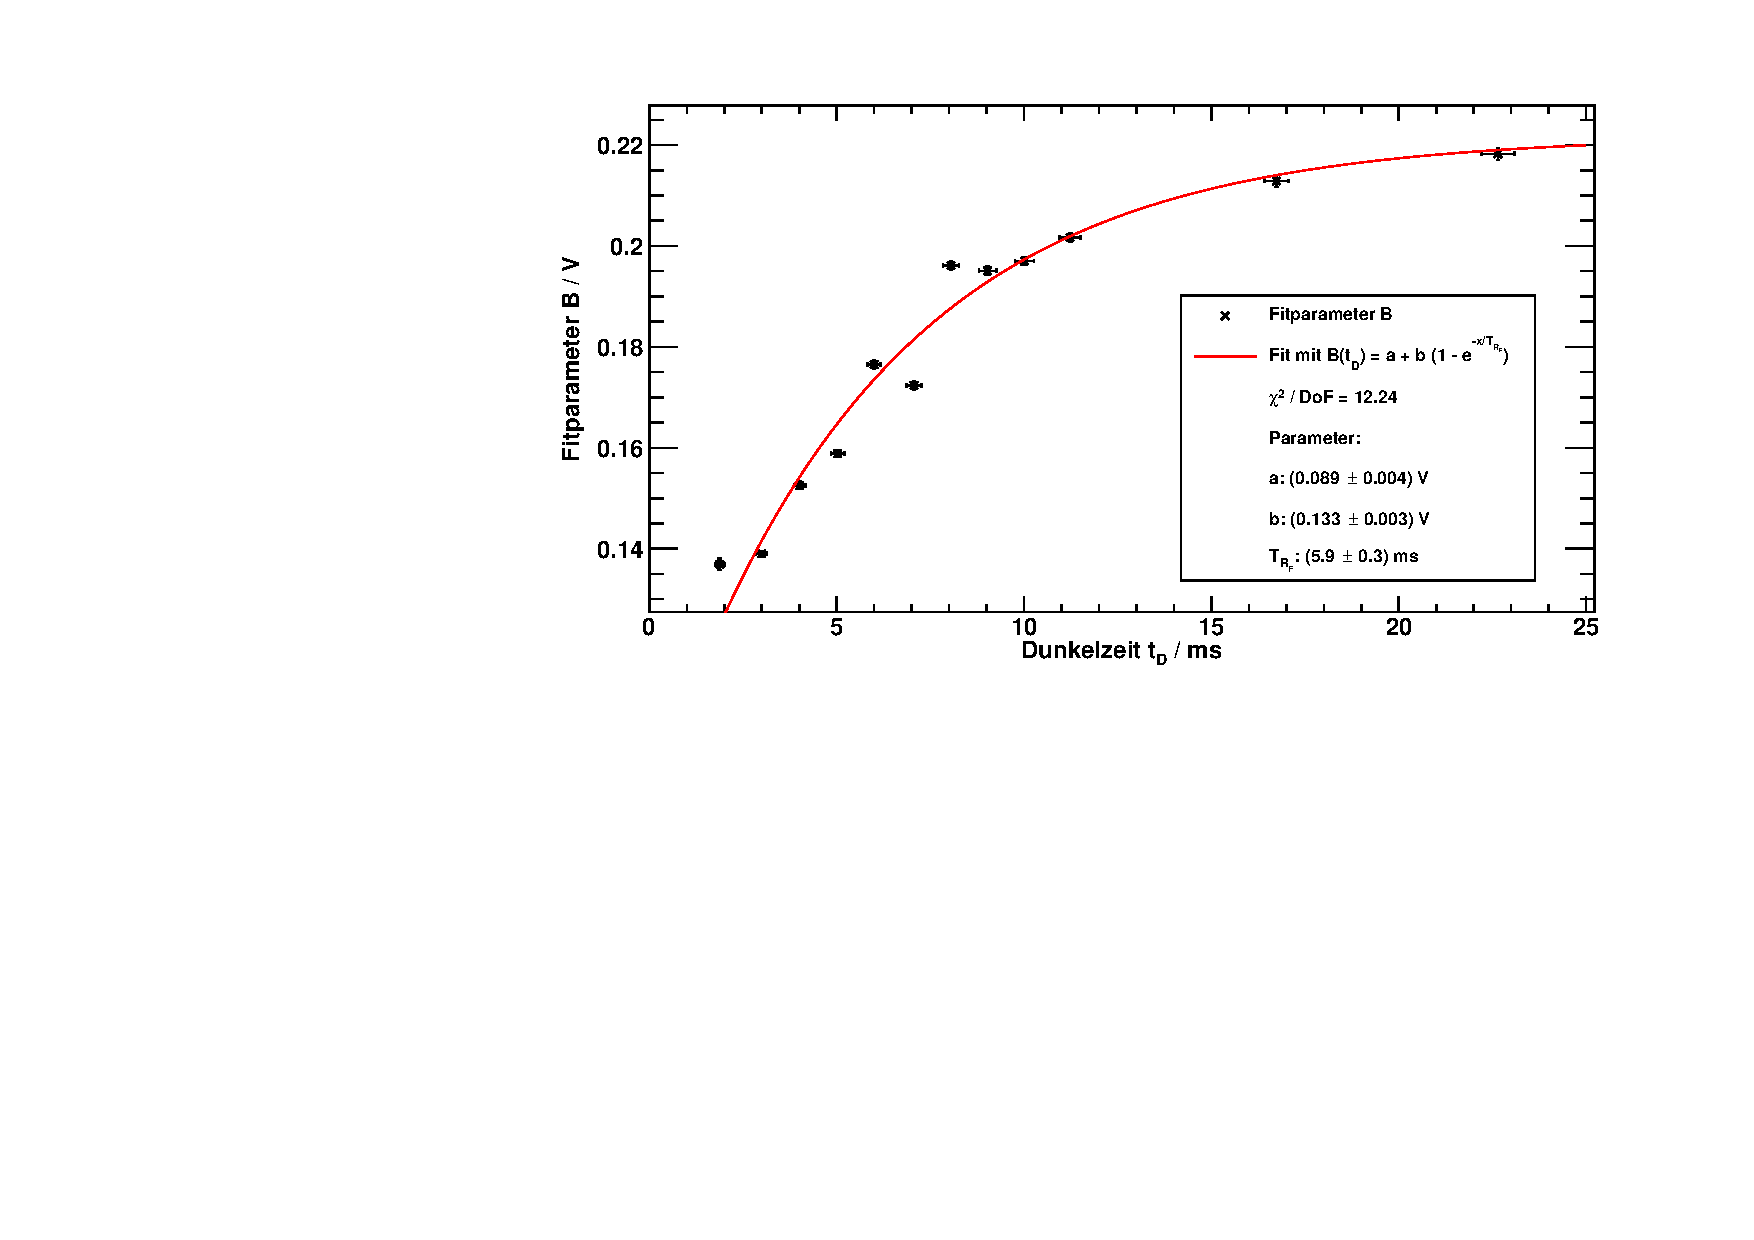
\includegraphics[width=\textwidth]{../img/BFit.pdf}
    \caption{Startwerte der gefitteten Exponentialfunktionen.}  
\end{figure} 
  
\end{frame}


\begin{frame}
\frametitle{Ergebnis: Bestimmung der Relaxationszeit nach Franzen}
\begin{itemize}
    \item Relaxationszeit
    \begin{equation*}
        T_{\text{R}_\text{F}} = 5.9 \pm 0.3\,\text{ms}
    \end{equation*}
    \item Literaturwert
    \begin{equation*}
        T_{\text{R}}^\text{Lit.} = 6.5\,\text{ms}
    \end{equation*}
\end{itemize}
  
\end{frame}
%
\section{Introduction}

\subsection[Short First Subsection Name]{First Subsection Name}

\begin{frame}
\frametitle{}
\framesubtitle{Subtitles are optional}

\begin{itemize}
  \item
  \item
\end{itemize}
\end{frame}

\begin{frame}
\frametitle{}

% You can create overlays
\begin{itemize}
  \item using the \texttt{pause} command:
  \begin{itemize}
    \item First item.
    \pause
    \item Second item.
  \end{itemize}
  \item using overlay specifications:
  \begin{itemize}
    \item<3-> First item.
    \item<4-> Second item.
  \end{itemize}
  \item using the general \texttt{uncover} command:
  \begin{itemize}
    \uncover<5->{\item First item.}
    \uncover<6->{\item Second item.}
  \end{itemize}
\end{itemize}
\end{frame}

\section*{Summary}

\begin{frame}
\frametitle<presentation>{Summary}

\begin{itemize}
  \item The \alert{first main message} of your talk in one or two lines.
\end{itemize}

% The following outlook is optional.
\vskip0pt plus.5fill
\begin{itemize}
  \item Outlook
  \begin{itemize}
    \item Something you haven't solved.
    \item Something else you haven't solved.
  \end{itemize}
\end{itemize}
\end{frame}

\end{document}
